% !Mode:: "TeX:UTF-8"

%Composed by Y.B. TANG (ybtang21c@gmail.com), spring-2011
%tex distribution: Texlive / MikTex 2010
%recommended editer: Eclipse + Texlipse
%usage: compile with XeLatex

%option: red, brown, blue
% \documentclass[14pt,mathserif]{beamer}
% \documentclass[14pt]{beamer}
\documentclass[usepdftitle=false, 14pt, handout]{beamer} %无动画
% \documentclass[usepdftitle=false, 14pt]{beamer}

\usepackage{amsmath,amsfonts,amssymb,amsthm,bm}
% \usepackage{txfonts} %another style of math fonts
\usepackage{beamerthemesplit,color,graphics}
\usepackage{ulem} %erase line
\usepackage{esint} %any type of integral symbol
% \usepackage{yhmath} %圆弧帽:\wideparen{AB}

\usepackage{tcolorbox} %各种自定义的盒子
\tcbuselibrary{skins, breakable, theorems}

\usepackage{bbding}%各种五角星
% \FiveStar,\FiveStarOpen,\FiveStarLines,\FiveStarShadow
% \FiveStarOutline,\FiveStarCenterOpen,\FiveStarOpenDotted
% \FiveStarConvex,\FiveStarOutlineHeavy,\FiveStarOpenCircled

%==============XeCJK==============================
\usepackage[slantfont,boldfont,CJKchecksingle]{xeCJK}
\setmainfont{Times New Roman}
\setCJKmainfont[BoldFont={Adobe Heiti Std},
	ItalicFont={Adobe Kaiti Std},
    SlantedFont={Adobe Song Std},
%     BoldItalicFont={Weibei SC},
     BoldSlantedFont={Adobe Fangsong Std}
	]{Adobe Heiti Std}
\punctstyle{CCT}
\usepackage{xeCJKfntef}%汉字加点和可断行的下划线

\newCJKfontfamily[Wawa]\Wawati{Wawati SC}
\newCJKfontfamily[STLi]\stliti{STLiti}

%============== Chinese Font Config 2 ===================

% \usepackage{fontspec, xunicode, xltxtra}
% \usepackage{xeCJK}%中文字体
% 
% \setmainfont{Times New Roman}%缺省英文字体 Times New Roman
% \setCJKmainfont[ItalicFont={Adobe Kaiti Std}, 
% 	BoldFont={Adobe Heiti Std}]{Adobe Song Std}%衬线字体 缺省中文字体
% \setCJKsansfont{Adobe Heiti Std}%serif是有衬线字体sans serif无衬线字体。
% \setCJKmonofont{Adobe Fangsong Std}%中文等宽字体

%======== customer defined fonts and fontsize ============

% %-----------------------xeCJK下设置中文字体------------------------------%
%常用字体
\setCJKfamilyfont{song}{Adobe Song Std}				%Adobe宋 \song
\newcommand{\song}{\CJKfamily{song}}                
      
\setCJKfamilyfont{fsong}{Adobe Fangsong Std}			%adobe仿宋 \fsong
\newcommand{\fsong}{\CJKfamily{fsong}}

\setCJKfamilyfont{kai}{Adobe Kaiti Std}				%Adobe楷体 \kaiti
\newcommand{\kaiti}{\CJKfamily{kai}}

\setCJKfamilyfont{hei}{Adobe Heiti Std}				%Adobe黑体 \heiti
\renewcommand{\heiti}{\CJKfamily{hei}}

\setCJKfamilyfont{hwzs}{STZhongsong}				%华文中宋 \hwzs
\newcommand{\hwzs}{\CJKfamily{hwzs}}

\setCJKfamilyfont{yh}{Microsoft YaHei}				%微软雅黑 \msyh
\newcommand{\msyh}{\CJKfamily{yh}}

%其他字体
\setCJKfamilyfont{hwfs}{STFangsong}				%华文仿宋  hwfs
\newcommand{\hwfs}{\CJKfamily{hwfs}}

\setCJKfamilyfont{hwxh}{STXihei}					%华文细黑  hwxh
\newcommand{\hwxh}{\CJKfamily{hwxh}}

\setCJKfamilyfont{hwl}{STLiti}						%华文隶书  hwl
\newcommand{\hwls}{\CJKfamily{hwl}}

\setCJKfamilyfont{hwxw}{STXinwei}					%华文新魏  hwxw
\newcommand{\hwxw}{\CJKfamily{hwxw}}

\setCJKfamilyfont{hwxk}{STXingkai}					%华文行楷  hwxk
\newcommand{\hwxk}{\CJKfamily{hwxk}}

\setCJKfamilyfont{hwhp}{STHupo}					%华文琥珀   hwhp
\newcommand{\hwhp}{\CJKfamily{hwhp}}

\setCJKfamilyfont{wawati}{Wawati SC}				%娃娃体 wawati
\newcommand{\wawati}{\CJKfamily{wawati}}

%------------------------------设置字体大小------------------------%
\newcommand{\chuhao}{\fontsize{42pt}{\baselineskip}\selectfont}     %初号
\newcommand{\xiaochuhao}{\fontsize{36pt}{\baselineskip}\selectfont} %小初号
\newcommand{\yihao}{\fontsize{28pt}{\baselineskip}\selectfont}      %一号
\newcommand{\erhao}{\fontsize{21pt}{\baselineskip}\selectfont}      %二号
\newcommand{\xiaoerhao}{\fontsize{18pt}{\baselineskip}\selectfont}  %小二号
\newcommand{\sanhao}{\fontsize{15.75pt}{\baselineskip}\selectfont}  %三号
\newcommand{\sihao}{\fontsize{14pt}{\baselineskip}\selectfont}%     四号
\newcommand{\xiaosihao}{\fontsize{12pt}{\baselineskip}\selectfont}  %小四号
\newcommand{\wuhao}{\fontsize{10.5pt}{\baselineskip}\selectfont}    %五号
\newcommand{\xiaowuhao}{\fontsize{9pt}{\baselineskip}\selectfont}   %小五号
\newcommand{\liuhao}{\fontsize{7.875pt}{\baselineskip}\selectfont}  %六号
\newcommand{\qihao}{\fontsize{5.25pt}{\baselineskip}\selectfont}    %七号

\usefonttheme{professionalfonts}

\newcommand{\fs}[1]{\fontspec{#1}\CJKfontspec{#1}}

%

% %==============std fontspec settings==============
% \usepackage[no-math,cm-default]{fontspec}
% % \newfontfamily\zhfont[BoldFont=Adobe Heiti Std]{Adobe Heiti Std}
% \newfontfamily\zhfont[BoldFont=Adobe Heiti Std]{Adobe Kaiti Std}
% % 
% % %==============spacing of CH in Xetex==============
% \usepackage{zhspacing}
% \zhspacing

%==============layout setting==============
\setlength{\parindent}{0pt}  

%==============beamer configuration==============
\setbeamertemplate{theorems}[normal font]

%============beamer theme setting #2============
\mode<presentation>{
	\usetheme{CambridgeUS} %Copenhagen, Warsaw, CambridgeUS
  	\usecolortheme{crane} %rose, seahorse, lily, crane
  	\usefonttheme{serif}
  	\usefonttheme{structurebold}
  	\useoutertheme{infolines}
%   \beamertemplateshadingbackground{brown!5}{yellow!10}
% 	\setbeamercolor{frametitle}{bg=white}	
%  	\setbeamercovered{transparent}
}

%============TOC setting============
% \AtBeginSection{
%    \begin{frame}{内容提要}
%      \tableofcontents[currentsection,hideallsubsections]
%    \end{frame}
% }
% \AtBeginSubsection{
%    \begin{frame}{内容提要}
%      \tableofcontents[currentsection,currentsubsection]
%    \end{frame}
% }
% \AtBeginSection{
%   \frame{\tableofcontents[sections={\thesection}]}
% }

%===============macros====================
% \newcommand{\bb}{\bf\color{blue}}
% \newcommand{\ba}[1]{\alert{\bf #1}}
% \newcommand*{\e}{\ensuremath{\varepsilon}}
% \renewcommand{\b}{\color{blue}}
% \newcommand*{\p}{\ensuremath{\partial}}
% \newcommand{\limn}{\ensuremath{\lim\limits_{n\to\infty}}}
% \newcommand{\sumn}{\ensuremath{\sum\limits_{n=1}^{\infty}}}
% \newcommand*{\df}[2]{\displaystyle\frac{\,{#1}\,}{\,{#2}\,}}
% \newcommand*{\limx}[1]{\ensuremath{\lim\limits_{x\to{#1}}}}
% \newcommand*{\limdx}{\ensuremath{\lim\limits_{\Delta x\to 0}}}
% \newcommand*{\dx}{\Delta x}
% \newcommand{\dint}{\ensuremath{\displaystyle\int}}
% \renewcommand{\d}{\mathrm{d}}
% \newcommand{\ds}{\displaystyle}

%===============macros====================
\def\ds{\displaystyle}
\def\fin{\hfill$\Box$}
\def\bs{\bigskip}
\def\b{\color{blue!80!yellow}}
\def\bb{\bf\color{blue}}
\def\e{\ensuremath{\varepsilon}}

\newcommand{\ba}[1]{\alert{\bf #1}}
\providecommand{\mbb}[1]{\ensuremath{\mathbb{{#1}}}}
\providecommand{\mr}[1]{\ensuremath{\mathrm{{#1}}}}


\newcommand{\limn}{\ensuremath{\lim\limits_{n\to\infty}}}
\newcommand*{\limx}[1]{\ensuremath{\lim\limits_{x\to{#1}}}}
\newcommand*{\limdx}{\ensuremath{\lim\limits_{\Delta x\to 0}}}
\providecommand{\llim}[1]{\ensuremath{\lim\limits_{#1}}}

\newcommand{\sumn}{\ensuremath{\sum\limits_{n=1}^{\infty}}}
\providecommand{\sumk}[1]{\ensuremath{\sum\limits_{k={#1}}^n}}
\providecommand{\suml}{\ensuremath{\sum\limits}}

\newcommand*{\df}[2]{\displaystyle\frac{\,{#1}\,}{\,{#2}\,}}
\newcommand*{\dx}{\Delta x}
\renewcommand{\d}{\mathrm{d}}
\newcommand*{\p}{\ensuremath{\partial}}

\newcommand{\dint}{\ensuremath{\displaystyle\int}}

\newcommand{\ps}[1]{$^{[\mbox{\it\footnotesize 注}]}$
\marginpar{\kaiti\small {注:}#1}}

%define tab of .25 textwidth and can auto strech
%\tab{the word}\tab{another word}\tab{3rd one}
\newlength{\tabcont}
\newcommand{\tab}[1]{%
	\settowidth{\tabcont}{#1}%
	\ifthenelse{\lengthtest{\tabcont < .25\linewidth}}%
	{\makebox[.25\linewidth][l]{#1}\ignorespaces}%
	%{\makebox[.5\linewidth][l]{\color{red} #1}\ignorespaces}%
	{\makebox[.5\linewidth][l]{#1}\ignorespaces}%
}%

%set fontsize with number of points
% \newcommand{\fs}[1]{\fontsize{#1 pt}{5pt}\selectfont}

\newtcolorbox{thx}{colframe=blue!40!black,colback=white,breakable}

\newtcolorbox{ext}{colframe=green!60!black,colback=green!20!white,breakable}



%================exampleblock counter===================
% \newcounter{examplecounter}
% \usecounter{examplecounter}
% \setcounter{examplecounter}{1}
% \newcommand{\exno}{{\bf
% 例\arabic{examplecounter}}\refstepcounter{examplecounter}}

%================block setting test=====================
% \definecolor{beamer@blendedred}{rgb}{0.7,0.2,0.2} % use structure theme to change
% \definecolor{beamer@blendedblue}{rgb}{0.2,0.2,0.7} % use structure theme to change
% \definecolor{beamer@blendedyellow}{rgb}{0.7,0.7,0.2}

% \setbeamercolor{structure}{fg=beamer@blendedred}

% \setbeamercolor{block title}
% {use=structure,fg=structure.fg,bg=structure.fg!20!bg}
% \setbeamercolor{block title alerted}
% {use=alerted text,fg=alerted text.fg,bg=alerted text.fg!20!bg}
% \setbeamercolor{block title example}
% {use=example text,fg=example text.fg,bg=example text.fg!20!bg}

% \setbeamercolor{block body}
% {parent=normal text,use=block title,bg=block title.bg!50!bg}
% \setbeamercolor{block body alerted}
% {parent=normal text,use=block title alerted,bg=block title alerted.bg!50!bg}
% \setbeamercolor{block body example}
% {parent=normal text,use=block title example,bg=block title example.bg!50!bg}

% \setbeamercolor{titlelike}{parent=structure,bg=white!90!red}
%=======================================================

%===============title setting====================

% \title{Advanced Mathematics II}
% \author[ybtang@nudt.edu.cn]{唐扬斌\\
% \texttt{\small ybtang21c@gmail.com\\tangyangbin@gfkd.mtn\\CP: 18374857376}}
% \institute[NUDT]{National University of Defense Technology}
% \date[Spring 2017]{Spring 2017}

\title{作业讲评}

%===============document begins here==============

\begin{document}

% % !Mode:: "TeX:UTF-8"

\titlepage

\begin{frame}{说在前面}
	\linespread{1.5}
	  \begin{itemize}[<+-|alert@+>]
	    \item 作业中打$\color{red}\times$的必须订正,否则下次不予批改,
		默认评分为$C$以下;
	    \item 写过的作业不许撕掉,除非重写;
	    \item 不要忘记贴照片,作业本封面注明学员队和班号;
	    \item 作业本不要分栏写;
	    \item 抄作业也要动脑子,不要当“复印机”!
	    \item {\b 今后每周一交作业,按照单双周对应学号尾数为单双号的同学分别上交,
	    平均每人两周交一次作业。} 
	  \end{itemize}
\end{frame}

\begin{frame}{出现的问题}
	\linespread{1.5}
	  \begin{itemize}[<+-|alert@+>]
	    \item 解题过程叙述不清,无用的话太多,未说明推理的依据;
	    \item 概念使用不熟练,例如:一道题里出现多个$\e$,不会正确地表达无界,无穷大;
	    \item 放缩不熟练,例如:$N$的取值太复杂;
	    \item 使用了不存在或无意义的极限,例如:$\limx0\sin\df1x$;
	    \item 符号书写不规范,如:$\mathbb{Z},\;\e,\;\delta$;
	    \item 书写脏乱,字迹难以辨认。
	  \end{itemize}
\end{frame}

\section{习题1-1}

\begin{frame}
	\linespread{1.5}
	\ba{5.用定义证明极限:(1)$\limn\df{\sqrt{n^2+a^2}}n=1$}\pause
	
	\bigskip
	
	证:\it 对任意$\e>0$,令$N=\left[\df{a^2}{\e}\right]+1>\df{a^2}{\e}$,
	则对任意$n>N$,均有
	$$\left|\df{\sqrt{n^2+a^2}}n-1\right|
	=\df{a^2}{n(\sqrt{n^2+a^2}+n)}<\df{a^2}n<\df{a^2}N<\e,
	$$
	由数列极限的定义,即证。\hfill$\Box$
\end{frame}

\begin{frame}
	\linespread{1.5}
	\ba{5.用定义证明极限:(4)$\limn0.\underbrace{99\ldots9}
	_{n\mbox{\footnotesize 个}}=1.$}\pause
	
	\bigskip
	
	证:\it 对任意$\e>0$,令$N=[-\lg\e]+1$,则对任意$n>N$,均有
	$$|0.\underbrace{99\ldots9}_{n\mbox{\footnotesize 个}}-1|
	=\df1{10^n}<\df1{10^N}
	<\df1{10^{-\lg\e}}=\e,$$
	由数列极限的定义,即证。\hfill$\Box$
\end{frame}

\begin{frame}
	\linespread{1.2}
	\ba{7.数列$\{x_n\}$有界,$\limn y_n=0$,证明:$\limn x_ny_n=0$。}\pause
	
	\bigskip
	
	证:\it $\{x_n\}$有界,故存在$M>0$,对任意$n\in\mathbb{Z}_+$,均有
	$$|x_n|\leq M.$$\pause
	对任意$\e>0$,令$\e_1=\df{\e}M$,由$\limn y_n=0$,存在$N$,对任意$n>N$有
	$$|y_n-0|<\e_1.$$\pause
	综上,当$n>N$时,总有
	$$|x_ny_n-0|\leq M\e_1=\e,$$
	由数列极限的定义,即证。\hfill$\Box$
\end{frame}

\begin{frame}
	\linespread{1.2}
	\ba{8.对于数列$\{x_n\}$,若$x_{2k-1}\to a\,(k\to\infty)$,
	$x_{2k}\to a\,(k\to\infty)$,证明:
	$x_n\to a\,(n\to\infty)$。}\pause
	
	\bigskip
	
	证:\it 对任意$\e>0$,由$x_{2k-1}\to a\,(k\to\infty)$,存在$K_1$,
	对任意$k>K_1$,有$|x_{2k-1}-a|<\e$;\pause
	对以上的$\e>0$,由$x_{2k}\to a\,(k\to\infty)$,存在$K_2$,
	对任意$k>K_2$,有$|x_{2k}-a|<\e$。\pause
	
	综上,令$N=\max\{2K_1-1,2K_2\}$,则对任意$n>N$,均有
	$$|a_n-a|<\e.$$
	由数列极限的定义,即证。\hfill$\Box$
\end{frame}

\section{习题1-3}

\begin{frame}
	\linespread{1.5}
	\ba{5.根据函数极限的定义证明:(3)$\limx{-2}\df{x^2-4}{x+2}=-4$.}\pause
	
	\bigskip
	
	证:\it 对任意$\e>0$,令$\delta=\e$,则对任意$x\in U_0(-2,\delta)$,总有
	$$\left|\df{x^2-4}{x+2}-(-4)\right|=|x+2|<\delta=\e.$$
	由函数极限的定义,即证。\hfill$\Box$
\end{frame}

\begin{frame}
	\linespread{1.5}
	\ba{6.根据函数极限的定义证明:
	(2)$\limx{+\infty}\df{\sin x}{\sqrt x}$.}\pause
	
	\bigskip
	
	证:\it 对任意$\e>0$,令$X=\df1{\e^2}$,则对任意$x>X$,总有
	$$\left|\df{\sin x}{\sqrt x}-0\right|\leq\df1{\sqrt x}
	<\df1{\sqrt X}=\e.$$
	由函数极限的定义,即证。\hfill$\Box$
\end{frame}

\begin{frame}
	\linespread{1.2}
	\ba{7.当$x\to2$时,$y=x^2\to 4$,问$\delta$等于多少,使当$|x-2|<\delta$时,
	$|y-4|<0.001$?}\pause
	
% 	\bigskip
	
	解:\it $$|y-4|<0.001\quad\Leftrightarrow\quad 3.999<x^2<4.001.$$
	进而当$x>0$时,必有
	$\sqrt{3.999}<x<\sqrt{4.001}$。	由此可知须
	$$|x-2|<\min\{2-\sqrt{3.999},\sqrt{4.001}-2\}$$
	时,方能满足题目要求。注意到$2-\sqrt{3.999}>\sqrt{4.001}-2$,故
	取$\delta=\sqrt{4.001}-2$,即为所求。\hfill$\Box$
\end{frame}

\begin{frame}
	\linespread{1.5}
	\ba{8.当$x\to\infty$时,$y=\df{x^2-1}{x^2+3}\to1$,问$X$等于多少,使当
	$|x|>X$时,$|y-1|<0.01$?}\pause
	
	\bigskip
	
	解:\it 由题意
	$$|y-1|=\left|\df{x^2-1}{x^2+3}-1\right|=\df4{x^2+3}<0.01,$$
	由此可解得$|x|>\sqrt{397}$,故$X=\sqrt{397}$即为所求。\hfill$\Box$
\end{frame}

\section{习题1-4}

\begin{frame}
	\linespread{1.5}
	\ba{7.证明:函数$y=\df1x\sin\df1x$在区间$(0,1]$内无界,但不是$x\to0^+$
	时的无穷大。}\pause
	
	\bigskip
	
	证:\it 先证该函数无界。对任意$M>0$,总可令$x_M=\df1{2([M]+1)\pi+\frac{\pi}2}$,
	则
	$$
	y(x_M)=2([M]+1)\pi+\frac{\pi}2>M.$$
	由函数无界的定义,即证。
\end{frame}

\begin{frame}
	\linespread{1.2}
	\ba{7.证明:函数$y=\df1x\sin\df1x$在区间$(0,1]$内无界,但不是$x\to0^+$
	时的无穷大。}\pause
	
	\bigskip
	
	\it 下证该函数不是$x\to0^+$时的无穷大。用反证法,若该函数是$x\to0^+$时的
	无穷大,则
	$$\limx{0^+}\df1y=\limx{0^+}x\df1{\sin\frac1x}=0.$$
	考虑数列$x_n=\frac1{n\pi}$,显然$\limn x_n=0$,且$\sin\df1{x_n}=0$,
	此时$\df1{y(x_n)}$无定义,故$\left\{\df1{y(x_n)}\right\}$
	必不收敛,从而由Henie定理,前述极限不成立,
	假设错误,即证。\hfill$\Box$
\end{frame}

\begin{frame}
	\linespread{1.5}
	\ba{8.求函数$f(x)=\df4{2-x^2}$的渐近线。}\pause
	
	\bigskip
	
	解:\it 由$\limx{\pm\sqrt 2}\df1{f(x)}=\df{2-x^2}4=0$,可知$f(x)$
	是$x\to\pm\sqrt2$时的无穷大,故$x=\pm\sqrt2$为$f(x)$的两条铅直渐近线;
	
	又$\limx{\infty}f(x)=0$,故$y=0$是$f(x)$的水平渐近线。\hfill$\Box$
\end{frame}

\section{习题1-5}

\begin{frame}
	\linespread{1.5}
	\ba{3.计算下列极限:(1)$\limx0x^2\sin\df1x$}\pause
	
	\bigskip
	
	解:\it 因为$\limx0x^2=0$,$|\sin\df1x|\leq1$,由无穷小的性质(无穷小
	乘以有界量仍为无穷小),可知
	$$\limx0x^2\sin\df1x=0.$$
	\hfill$\Box$
\end{frame}

\begin{frame}
	\linespread{1.5}
	\ba{3.计算下列极限:(2)$\limx{\infty}\df{\arctan x}x$}\pause
	
	\bigskip
	
	解:\it 因为$\limx{\infty}\df1x=0$,$|\arctan x|\leq\df{\pi}2$,故
	无穷小的性质,可知
	$$\limx{\infty}\df{\arctan x}x=0.$$
	\hfill$\Box$
\end{frame}

% % !Mode:: "TeX:UTF-8"

\titlepage

\begin{frame}{说在前面}
	\linespread{1.5}
	  \begin{itemize}[<+-|alert@+>]
	    \item 过往的作业只画$\color{red}\times$和划线,不画$\color{red}\surd$,
	    最后写{\bb “查”};
	    \item 就近订正,方便查阅,用不同颜色的笔;
	    \item 不要忘记贴照片,作业本封面注明学员队和班号!
	    \item 作业本不要分栏写!
	    \item 不要当“复印机”!
	    \item 作业晚交、进度过慢或缺题过多最高得$\b B$,
	    不交默认为$\b C$!
% 	    \item {\b 今后每周一交作业,按照单双周对应学号尾数为单双号的同学分别上交,
% 	    平均每人两周交一次作业。} 
	  \end{itemize}
\end{frame}

\begin{frame}{出现的问题}
	\linespread{1.5}
	  \begin{itemize}[<+-|alert@+>]
	    \item 口语化的表达
	    \begin{itemize}
	      \item {\it\b $f(x)$在\ldots附近,两头收敛}
	      \item {\it\b $x=0$附近的情况与$x=2$附近的情况相同}
	    \end{itemize}
	    \item 概念错误
	    \begin{itemize}
	      \item {\it\b $\limx0f(x)=\limx0\sin x$,故$\limx0\df{f(x)}{\sin x}=1$}
	      \item {\it\b $f'_+(0)=\limx{0^+}f'(x)$} 
	    \end{itemize}
	    \item 自己发明符号
		$$\b y'_{x\to 0^+},\quad f'(x)_{\mbox{\footnotesize\it 左}},
		\quad f\left.\left(\arctan\df{1+x}{1-x}\right)'\right|_{x=0}$$
	  \end{itemize}
\end{frame}

\section{习题1-9}

\begin{frame}
	\linespread{1.5}
	\ba{2.设函数$f(x)$与$g(x)$在点$x_0$连续,证明函数
	$$\varphi(x)=\max\{f(x),g(x)\},\quad
	\psi(x)=\min\{f(x),g(x)\}$$
	在$x_0$也连续。}\pause
	
% 	\bigskip
	
	证:\it
	$$\max\{f(x),g(x)\}=\df12[f(x)+g(x)+|f(x)-g(x)|],$$
% 	$$\min\{f(x),g(x)\}=\df12[f(x)+g(x)-|f(x)-g(x)|],$$
	\pause 由已知,$\limx{x_0}f(x)=f(x_0),
	\limx{x_0}g(x)=g(x_0),$
	\pause 进而由极限的性质可得
	$$\limx{x_0}|f(x)-g(x)|=|f(x_0)-g(x_0)|,$$
\end{frame}

\begin{frame}
	\linespread{1.5}
% 	\ba{2.设函数$f(x)$与$g(x)$在点$x_0$连续,证明函数
% 	$$\varphi(x)=\max\{f(x),g(x)\},\quad
% 	\psi(x)=\min\{f(x),g(x)\}$$
% 	在$x_0$也连续。}\pause
	
% 	\bigskip
	
	\it\small 于是
	\begin{align*}
		\limx{x_0}\varphi(x)&=\limx{x_0}\max\{f(x),g(x)\}\\
		&=\limx{x_0}\df12[f(x)+g(x)+|f(x)-g(x)|]\\
		&=\df12\left[\limx{x_0}f(x)+\limx{x_0}g(x)+\limx{x_0}|f(x)-g(x)|\right]\\
		&=\df12[f(x_0)+g(x_0)+|f(x_0)-g(x_0)|]\\
		&=\max\{f(x_0),g(x_0)\}=\varphi(x_0).
	\end{align*}
	\pause 也即 $\varphi(x)$在$x_0$连续。
	\pause
	$$\psi(x)=\min\{f(x),g(x)\}=\df12[f(x)+g(x)-|f(x)-g(x)|],$$
	同理可证$\psi(x)$在$x_0$连续。\hfill$\Box$
\end{frame}

\section{习题1-10}

\begin{frame}
	\linespread{1.5}
	\ba{7.证明:若$f(x)$在$(-\infty,+\infty)$内连续,且$\limx{\infty}f(x)$
	存在,则$f(x)$必在$(-\infty,+\infty)$内有界。}\pause
	
% 	\bigskip
	
	证:\it
	$\limx{\infty}f(x)$存在,由极限的有界性,$\exists M_1>0$和$X>0$,
	对$\forall |x|>X$,均有$|f(x)|\leq M_1$。
	\pause
	注意到$f(x)\in C[-X,X]$,故$\exists M_2>0$,对$\forall x\in[-X,X]$,
	均有$|f(x)|\leq M_2$。
	\pause
	综上,对任意$x\in(-\infty,+\infty)$,均有
	$$|f(x)|\leq M=\max\{M_1,M_2\}.$$
	即证。\hfill$\Box$
\end{frame}

\section{总习题一}

\begin{frame}
	\linespread{1.5}
	\ba{14.如果存在直线$L:y=kx+b$,使当$x\to+\Delta$时
	($\Delta$表示$\infty,+\infty,-\infty$之一),
	曲线$y=f(x)$上的动点$M(x,y)$到直线$L$的距离
	$d(M,L)\to 0$,那么称$L$为直线$y=f(x)$的渐近线。当直线$L$的斜率
	$k\ne 0$时,称$L$为斜渐近线。
	\begin{enumerate}[(1)]
% 	  \setlength{\itemindent}{1cm}
	  \item 证明:直线$L:y=kx+b$为曲线$y=f(x)$的渐近线的充分必要条件是
	  $$k=\limx{\Delta}\df{f(x)}x,\quad
	  b=\limx{\Delta}[f(x)-kx].$$
	  \item 求曲线$y=(2x-1)e^{\frac1x}$的斜渐近线。
	\end{enumerate}}
\end{frame}

\section{1.2 导数的概念}

\begin{frame}
	\linespread{1.5}
	\ba{1.已知$f(x)=\left\{\begin{array}{ll}
	2e^x+b,& x\leq0\\ ax+\sin x,& x> 0
	\end{array}\right.$
	试确定$a,b$的值,使得$f(x)$在$x=0$处可导。}\pause
	
% 	\bigskip
	
	\small 证:\it
	$f(x)$在$x=0$处可导,故必连续,从而
	$$f(0-0)=2+b=f(0+0)=0\quad\Rightarrow \quad b=-2.$$
	\pause 又
	$$f'_-(0)=(2e^x+b)'|_{x=0}=2.$$
	$$f'_+(0)=\limx{0^+}\df{ax+\sin x-(2+b)}{x}
	=a+\limx{0^+}\df{\sin x}x=a+1.$$
	故要使$f(x)$在$x=0$处可导,必有$2=a+1$,从而$a=1$。
	\hfill$\Box$
\end{frame}

\begin{frame}
	\linespread{1.5}
	\ba{3.讨论函数
	$y=\left\{\begin{array}{ll}
		x^2\sin\df1x,& x\ne0;\\ 0, & x=0.
	\end{array}\right.$
	在$x=0$处的连续性、可导性以及导函数的连续性。}\pause
	
% 	\bigskip
	
	\small 证:\it
	当$x\ne 0$时,
	$$y'(x)=2x\sin\df1x-\sin\df1x.$$
	\pause 当$x=0$时,
	$$y'(0)=\limx0\df{x^2\sin\df1x-0}{x-0}=\limx0x\sin\df1x=0.$$
	由此可知$y(x)$在$x=0$处可导,且连续。
\end{frame}

\begin{frame}
	\linespread{1.5}
	\small\it
	$$
		y'=\left\{\begin{array}{ll}
			2x\sin\df1x-\sin\df1x, & x\ne 0,\\
			0, & x=0.
		\end{array}\right.
	$$
	\pause
	注意到
	$$\limx02x\sin\df1x=0,\quad \limx0\sin\df1x\mbox{不存在},$$
	故$\limx0y'(x)$不存在。由此可知$y(x)$的导函数在$x=0$处不连续。\hfill$\Box$
	
	\bigskip
	\pause 
	\ba{注:可导函数的导函数不一定是连续函数!}
\end{frame}

\begin{frame}
	\linespread{1.5}
	\ba{4.设对任意$x\in\mathbb{R}$,均有$f(x+2)=f(x)$,已知$f'(0)=1$,
	证明$f(x)$在$x=2$可导,并求$f'(2)$。}\pause
	
	\bigskip
	
	\small 解:\it
	因为$f(x+2)=f(x)$,故
	$$\lim\limits_{\Delta x\to0}\df{f(2+\Delta x)-f(2)}{\Delta x}
	=\lim\limits_{\Delta x\to0}\df{f(\Delta x)-f(0)}{\Delta x}
	=f'(0)=1,$$
	由此即知$f(x)$在$x=2$可导,且$f'(2)=1$。
	\hfill$\Box$
	
	\bigskip
	\pause
	\ba{注:周期函数的导函数必为周期函数,反之不然。}
\end{frame}

\begin{frame}
	\linespread{1.5}
	\ba{5.已知曲线$y=f(x)$和曲线$y=\sin x$在原点相切(即二者的切线相同),
	求$\limx0\df{f(3x)}x$。}\pause
	
	\bigskip
	
	\small 解:\it
	曲线$y=f(x)$和曲线$y=\sin x$在原点相切,故
	$$f(0)=\sin 0=0,\quad f'(0)=(\sin x)'|_{x=0}=1.$$
	于是
	$$\limx0\df{f(3x)}x=3\limx0\df{f(3x)-f(0)}{3x}=3f'(0)=3.$$
	\hfill$\Box$
\end{frame}

\begin{frame}
	\linespread{1.5}
	\ba{6.函数$g(x)$在$x=a$连续,问函数$f(x)=|(x-a)|g(x)$
	在$x=a$是否可导?若可导,证明之;若不可导,讨论增加什么样的条件可以使之可导。
	利用以上讨论的结果,判断$f(x)=(x^2-4)|x^2+3x+2|$有几个不可导的点。}\pause
	
% 	\bigskip
	
	\small 解:\it
	$$\df{f(a+\Delta x)-f(a)}{\Delta x}
	=\df{|\Delta x|g(a+\Delta x)}{\Delta x}
	=\df{|\Delta x|}{\Delta x}g(a+\Delta x),$$
	\pause
	当$\Delta x\to0$时极限存在当且仅当$\lim\limits_{\Delta x\to0}g(a+\Delta x)=0$,也即
	$\limx{a}g(x)=0$。
	\pause
	$f(x)=|(x+2)(x+1)|(x+2)(x-2),$
	根据前述的结论,在$x=-2$处$f(x)$可导,在$x=-1$处$f(x)$不可导。\hfill$\Box$
\end{frame}

\begin{frame}
	\linespread{1.5}
	\ba{7.已知$f'(a)f(a)\ne 0$,求
	$\limx0\left[\df{f(a+x)}{f(a)}\right]^{\frac1{\sin x}}.$}\pause
	
% 	\bigskip
	
	\small 解:\it
	\begin{align*}
		\mbox{原式}&=\limx0\left[1+\df{f(a+x)-f(a)}{f(a)}\right]^{\frac1{\sin x}}\\
		&=\limx0\left[1+\df{f(a+x)-f(a)}{f(a)}\right]^{\frac{f(a)}{f(a+x)-f(a)}
		\frac{f(a+x)-f(a)}{f(a)}\frac1{\sin x}}\\
		&=\left\{\limx0\left[1+\df{f(a+x)-f(a)}{f(a)}\right]^{\frac{f(a)}{f(a+x)-f(a)}}\right\}
		^{\limx0\frac{f(a+x)-f(a)}x\frac{x}{\sin x}\frac1{f(a)}}\\
		&=e^{\frac{f'(a)}{f(a)}}
	\end{align*}
	\hfill$\Box$
\end{frame}

\begin{frame}
	\linespread{1.5}
	\ba{8.设对任意$x,y\in\mathbb{R}$,有
	$$f(x+y)=f(x)+f(y)+x^2y+xy^2,$$
	且当$x\to0$时$f(x)$与$x$是等价无穷小,证明$f(x)$处处可导,并求其导函数。}\pause
	
% 	\bigskip
	
	\small 解:\it
	令$x=y=0$,由已知等式可得$f(0)=0$。\pause
	对任意$x_0\in\mathbb{R}$,由已知等式及$\limx{0}\df{f(x)}x=1$,
	\begin{align*}
		\lim\limits_{\Delta x\to0}\df{f(x_0+\Delta x)-f(x_0)}{\Delta x}
		&=\lim\limits_{\Delta x\to0}\df{f(\Delta x)+x_0^2\Delta x+x_0\Delta x^2}
		{\Delta x}\\
		&=\lim\limits_{\Delta x\to0}\df{f(\Delta x)}{\Delta x}+x_0^2
		=1+x_0^2.
	\end{align*}
	\pause 因为$x_0$是任意的,故$f(x)$处处可导,其导函数为
	$f'(x)=1+x^2$。\hfill$\Box$
\end{frame}

\section{2.2 函数的求导法则}

\begin{frame}
	\linespread{1.5}
	\ba{4.设$f(x)$可导,且$f'\left(\df{\pi}{4}\right)=1$,求
	$$\left.f'\left(\arctan\df{1+x}{1-x}\right)\right|_{x=0}
	\quad\mbox{和}\quad  
	\left[f\left(\arctan\df{1+x}{1-x}\right)\right]'_{x=0}.$$}\pause
	
% 	\bigskip
	
	\small 解:\it
	$$\left.f'\left(\arctan\df{1+x}{1-x}\right)\right|_{x=0}
	=f'(\arctan 1)=f'\left(\df{\pi}{4}\right)=1.$$
	\pause
	\begin{align*}
		&\left[f\left(\arctan\df{1+x}{1-x}\right)\right]'_{x=0}
		=f'\left(\arctan\df{1+x}{1-x}\right)\\
		&\quad\left.\df{1}{1+\left(\frac{1+x}{1-x}\right)^2}
		\df{(1-x)+(1+x)}{(1-x)^2}
		\right|_{x=0}
		=1\cdot\df12\cdot2=1.
	\end{align*}
	\hfill$\Box$
\end{frame}

% % !Mode:: "TeX:UTF-8"

\titlepage

% \begin{frame}{说在前面}
% 	\linespread{1.5}
% 	  \begin{itemize}[<+-|alert@+>]
% 	    \item 过往的作业只画$\color{red}\times$和划线,不画$\color{red}\surd$,
% 	    最后写{\bb “查”};
% 	    \item 就近订正,方便查阅,用不同颜色的笔;
% 	    \item 不要忘记贴照片,作业本封面注明学员队和班号!
% 	    \item 作业本不要分栏写!
% 	    \item 不要当“复印机”!
% 	    \item 作业晚交、进度过慢或缺题过多最高得$\b B$,
% 	    不交默认为$\b C$!
% % 	    \item {\b 今后每周一交作业,按照单双周对应学号尾数为单双号的同学分别上交,
% % 	    平均每人两周交一次作业。} 
% 	  \end{itemize}
% \end{frame}

\begin{frame}{出现的问题}
	\linespread{1.5}
	  \begin{itemize}[<+-|alert@+>]
	    \item 求导题
	    \begin{itemize}
	      \item \b\it $y^n$和$y^{(n)}$混淆
	      \item \b\it 分段定义的函数分段点处的导数值没有用定义计算
	    \end{itemize}
	    \item 应用题
	    \begin{itemize}
	      \item \b\it $x'(t)=5$,故$x(t)=5t$ \ba{$\times$}
	      \item \b\it 无图无文字,让人如何看得懂?!
	    \end{itemize}
	  \end{itemize}
\end{frame}

\section{2.3 高阶导数}

\begin{frame}
	\linespread{1.5}
	\ba{2.已知$f(x)$二阶可导,设$y=\df{f(x)}{x}$,求$\df{\d^2y}{\d x^2}$。}
	\pause
	
% 	\bigskip
	
	解:\it
	\begin{align*}
		y'&=\df{f'(x)x-f(x)}{x^2},\\
		y''&=\df{f''(x)x^3-2x[f'(x)x-f(x)]}{x^4}\\
		&=\df{f''(x)x^2-2f'(x)x+2f(x)}{x^3}.
	\end{align*}
	\hfill$\Box$
\end{frame}

\begin{frame}
	\linespread{1.5}
	\ba{3.已知$f(x)=\left\{\begin{array}{ll}
	  	\ln(1+2x),& x>0, \\ x^2+2x, & x\leq 0,
	  \end{array}\right.$
	求$f''(x)$。}\pause
	
	\bigskip
	
	\small 解:\it 
	$x>0$时,$f'(x)=\df2{1+2x}$;$x<0$时,$f'(x)=2x+2$,
	\pause 又
	$$f'_-(0)=\lim\limits_{\Delta x\to0^-}\df{\Delta x^2+2\Delta x-0}{\Delta x}=2.$$
	$$f'_+(0)=\lim\limits_{\Delta x\to0^+}\df{\ln(1+2\Delta x)-0}{\Delta x}=2.$$
	故$f'(0)=2$。
\end{frame}

\begin{frame}
	\linespread{1.5}
% 	\ba{3.已知$f(x)=\left\{\begin{array}{ll}
% 	  	\ln(1+2x),& x>0, \\ x^2+2x, & x\leq 0,
% 	  \end{array}\right.$
% 	求$f''(x)$。}\pause
	
% 	\bigskip
	
	\small \it 
	进而,当$x>0$时,$f''(x)=-\df4{(1+2x)^2}$;当$x<0$时,$f''(x)=2$,
	\pause 又
	$$f''_+(0)=\lim\limits_{\Delta x\to0^+}
	\df{\frac2{1+2\Delta x}-2}{\Delta x}
	=\lim\limits_{\Delta x\to0^+}
	\df{-4}{1+2\Delta x}=-4,$$
	$$f''_+(0)=\lim\limits_{\Delta x\to0^+}
	\df{2\Delta x+2-2}{\Delta x}=2,
	$$
	故$f''(0)$不存在。综上
	$$f''(x)=\left\{\begin{array}{ll}
		-\df4{(1+2x)^2}, & x>0;\\
		2, & x<0.
	\end{array}\right.$$
	\hfill$\Box$
\end{frame}

\begin{frame}
	\linespread{1.5}
	\ba{4.求下列函数的$n$阶导函数:(1)$y=\sin^2x$}\pause
	
	\bigskip
	
	\small 解:\it
	$y=\df12(1-\cos2x)$,从而
	\begin{align*}
		y'&=\df12\cdot 2\sin2x,\\
		y''&=\df12\cdot 2^2\cos2x=2\sin\left(2x+\df{\pi}2\right),\\
		y'''&=2^2\cos\left(2x+\df{\pi}2\right)=2^2\sin\left(2x+2\cdot\df{\pi}2\right),\\
		\ldots&\ldots\\
		y^{(n)}&=2^{n-1}\sin\left(2x+(n-1)\cdot\df{\pi}2\right)
	\end{align*}
\end{frame}

\begin{frame}
	\linespread{1.5}
	\ba{4.求下列函数的$n$阶导函数:(2)$y=x\ln x$}\pause
	
	\bigskip
	
	\small 解:\it
	\begin{align*}
		y'&=\ln x+1,\\
		y''&=\df1x,\\
		y'''&=-\df1{x^2},\\
		y^{(4)}&=\df2{x^3},\\
		\ldots&\ldots\\
		y^{(n)}&=(-1)^n\df{(n-2)!}{x^{n-1}}.
	\end{align*}
\end{frame}

\begin{frame}
	\linespread{1.5}
	\ba{4.求下列函数的$n$阶导函数:(3)$y=\df{x^2}{1-x}$}\pause
	
	\bigskip
	
	\small 解:\it
	$y=-(x+1)+\df1{1-x}$,故
	\begin{align*}
		y'&=-1+\df1{(1-x)^2},\\
		y''&=\df2{(1-x)^3},\\
		y'''&=\df{2\cdot 3}{(1-x)^4},\\
		\ldots&\ldots\\
		y^{(n)}&=\df{n!}{(1-x)^{n+1}}.
	\end{align*}
\end{frame}

\begin{frame}
	\linespread{1.5}
	\ba{5.已知$f(x)=x^2\ln(1+x)$,求$f^{(n)}(0)$。}\pause
	
	\bigskip
	
	\small 解:\it
	由Leibniz公式,当$n\geq3$时,
	\begin{align*}
		&f^{(n)}(x)\\
		&=x^2[\ln(1+x)]^{(n)}+n2x[\ln(1+x)]^{(n-1)}
		+\df{n(n-1)}22[\ln(1+x)]^{(n-2)}\\
		&=x^2\df{(-1)^{n-1}(n-1)!}{(1+x)^n}+2nx\df{(-1)^{n-2}(n-2)!}{(1+x)^{n-1}}\\
		&\quad +n(n-1)\df{(-1)^{n-3}(n-3)!}{(1+x)^{n-2}}.
	\end{align*}
	\pause 令$x=0$,可得
	$$f^{(n)}(0)=(-1)^{n-1}\df{n!}{n-2}.$$
	\hfill$\Box$
\end{frame}

\section{2.4 隐函数与参数方程求导}

\begin{frame}
	\linespread{1.5}
	\ba{1.对下列函数,求$y''(x)$:(1)$y=\tan(x+y)$}\pause
	
% 	\bigskip
	
	\small 解:\it
	方程两边对$x$求导,可得
	$$y'=\sec^2(x+y)(1+y')=(1+y^2)(1+y'),$$
	\pause 整理后即为
	$$y'=-1-\df1{y^2}.$$
	\pause 两边再次对$x$求导,可得
	$$y''=\df{2y'}{y^3}=-\df2{y^3}\left(1+\df1{y^2}\right)
	=-2\df{\csc^2(x+y)}{y^3}.$$
\end{frame}

\begin{frame}
	\linespread{1.5}
	\ba{1.对下列函数,求$y''(x)$:(2)$y=1+xe^y$}\pause
	
% 	\bigskip
	
	\small 解:\it
	方程两边对$x$求导,可得
	$$y'=e^y(1+xe^yy'),$$
	也即
	$$y'=\df{e^y}{1-xe^y}=\df{e^y}{2-y}.$$
	\pause 两边再次对$x$求导,可得
	$$y''=e^y\df{y'(2-y)+1}{(2-y)^2}=\df{e^y(e^y+1)}{(y-2)^2}.$$
\end{frame}

\begin{frame}
	\linespread{1.5}
	\ba{3.已知$\left\{\begin{array}{l}
	  	x=e^t\cos t\\ y=e^t\sin t
	\end{array}\right.$,求$\left.\df{\d y}{\d x}\right|_{t=\frac{\pi}2}$
	和$\left.\df{\d^2 y}{\d x^2}\right|_{t=\frac{\pi}2}$。}\pause
	
% 	\bigskip
	
	\small 解:\it
	$$\df{\d y}{\d x}=\df{\df{\d y}{\d t}}{\df{\d x}{\d t}}
	=\df{\sin t+\cos t}{\cos t-\sin t}.$$
	当$t=\df{\pi}2$时,$y'_x=-1$。
	\pause 进一步,
	$$\df{\d^2 y}{\d x^2}
	=\df{\df{\d y'_x}{\d t}}{\df{\d x}{\d t}}
	=\df{2}{e^x(\cos t-\sin t)^3},$$
	从而$y''_{xx}|_{t=\frac{\pi}2}=-2e^{-\frac{\pi}2}$。\hfill$\Box$
\end{frame}

\begin{frame}
	\linespread{1.5}
	\ba{4.设$x(t),y(t)$均三阶可导,试给出$y'''_{xxx}$关于$t$的表达式。}\pause
	
	\bigskip
	
	\small 解:\it
	\begin{align*}
		y'_x&=\df{\d y}{\d x}=\df{\df{\d y}{\d t}}{\df{\d x}{\d t}}
		=\df{y'_t}{x'_t};\\
		y''_{xx}&=\df{\d y'_x}{\d x}=\df{\df{\d y'_x}{\d t}}{\df{\d x}{\d t}}
		=\df{\d }{\d t}\left(\df{y'_t}{x'_t}\right)\df{1}{x'_t}
% 		=\df{y''_{tt}x'_t-y'_tx''_{tt}}{(x'_t)^2}\df{1}{x'_t}
		=\df{y''_{tt}x'_t-y'_tx''_{tt}}{(x'_t)^3},\\
		y'''_{xxx}&=\df{\d y''_{xx}}{\d x}
		=\df{\df{\d y''_{xx}}{\d t}}{\df{\d x}{\d t}}
% 		=\df{\d }{\d t}\left(\df{y''_{tt}x'_t-y'_tx''_{tt}}{(x'_t)^3}\right)
% 		\df{1}{x'_t}\\
% 		&=\df{(y'''_{ttt}x'_t+y''_{tt}x''_{tt}
% 		-y''_{tt}x''_{tt}-y'_tx'''_{ttt})(x'_t)^3
% 		-(y''_{tt}x'_t-y'_tx''_{tt})3(x'_t)^2x''_{tt}}{(x'_t)^6}\df{1}{x'_t}\\
		=\df{(y'''_{ttt}x'_t-y'_tx'''_{ttt})x'_t
		-3(y''_{tt}x'_t-y'_tx''_{tt})x''_{tt}}{(x'_t)^5}.
	\end{align*}
	\hfill$\Box$
\end{frame}

\begin{frame}
	\linespread{1.5}
	\ba{5.设曲线的极坐标方程为$\rho=\rho(\theta)$,求其对应的直角指标
	方程$y=y(x)$相关的导数$y'_x$和$y''_{xx}$关于$\theta$的表达式。}\pause
	
	\bigskip
	
	\small 解:\it
	$x=\rho(\theta)\cos\theta,\;y=\rho(\theta)\sin\theta$,
	$$\df{\d y}{\d x}=\df{\df{\d y}{\d\theta}}{\df{\d x}{\d\theta}}
	=\df{\rho'\sin\theta+\rho\cos\theta}{\rho'\cos\theta-\rho\sin\theta},$$
	\pause
	进而
	$$\b
	\df{\d^2y}{\d x^2}
	=\df{\df{\d}{\d\theta}\left(\df{\d y}{\d x}\right)}{\df{\d x}{\d\theta}}
	=\df{\rho^2+2(\rho')^2-\rho\rho''}{(\rho'\cos\theta-\rho\sin\theta)^3}.
	$$
	\hfill$\Box$
\end{frame}

\section{2.5 相关变化率}

\begin{frame}
	\linespread{1.5}
	\ba{1.质点$P$沿抛物线$x=y^2(y>0)$移动。$P$的横坐标$x$的变化速度为$5$cm/s。
	当$x=9$cm时,点$P$到原点的距离的变化速率是多少?}\pause
	
% 	\bigskip
	
	\small 解:\it
	点$P(x,y)$到原点的距离$d=\sqrt{x^2+y^2}$,则
	$$\df{\d d}{\d t}=\df{\sqrt{x^2+y^2}}{\d t}
	=\df{xx'_t+yy'_t}{\sqrt{x^2+y^2}}.$$
	\pause 当$x=9$,$x'_t=5$时,
	$$
		y=3,\quad
		y'_t=\df{\d y}{\d x}{\df{\d x}{\d t}}
		=\df{x'_t}{x'_y}=\df5{2y}=\df56.
	$$
	带入前式,可得所求变化率为$\df{9\cdot 5+3\cdot\df56}{3\sqrt{10}}
	=\df{95}{6\sqrt{10}}$。\hfill$\Box$
\end{frame}

\begin{frame}
	\linespread{1.5}
	\ba{2.垂直向上发射一枚火箭,在其起飞点100km外设置一个观察站,在观察仰角
	为$\pi/4$时,测得仰角的增加率为$0.1$弧度每秒,求此时火车的上升速率。}\pause
	
% 	\bigskip
	
	\small 解:\it
	如图,
	\begin{columns}
		\column{0.4\textwidth}
		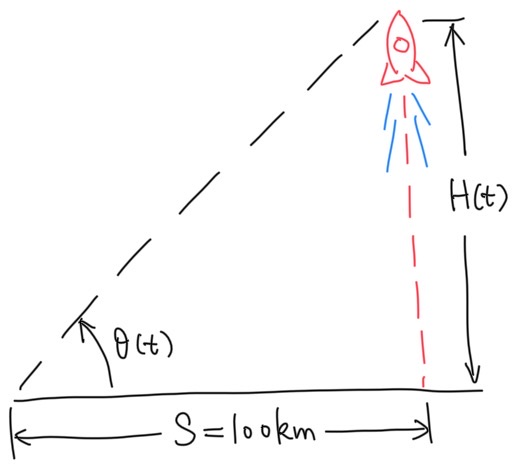
\includegraphics[width=5cm]{./images/ch2/Rocket.jpg}
		\column{0.6\textwidth}
		\pause 火箭的高度$H(t)=S\tan\theta(t)$,由此可知
		$$H'(t)=S\sec^2\theta(t)\theta'(t),$$
		\pause 将$S=100$,$\theta(t)=\df{\pi}4$,$\theta'(t)=0.1$代入即得
		指定时刻火箭上升的速率为$20$km/s。\hfill$\Box$
	\end{columns}
\end{frame}

\begin{frame}
	\linespread{1.5}
	\ba{3.长度为$6$米的梯子靠在墙角,梯子底部距离墙角$5$米,某一时刻梯子底部开始
	向远离墙角的方向滑动,滑动的速度为$0.2$米每秒,问
	\begin{enumerate}[(1)]
	  \setlength{\itemindent}{1cm}
	  \item 此时梯子顶部下滑的速度是多少?
	  \item 由梯子、墙面和地面构成的三角形的面积随时间的变化率是多少?
	  \item 梯子和地面的夹角的以怎样的速率变化?
	\end{enumerate}}	
\end{frame}

\begin{frame}
	\linespread{1.5}
	\small 解:\it
	如图,
	\begin{columns}
		\column{0.4\textwidth}
		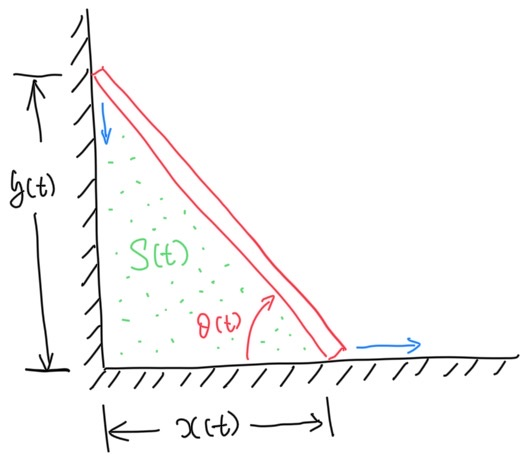
\includegraphics[width=5cm]{./images/ch2/ladder.jpg}
		\column{0.6\textwidth}
		\pause (1)显然$x^2(t)+y^2(t)=36$,两边求导可得
		$x'(t)x(t)+y'(t)y(t)=0$,进而
		$$y'(t)=-\df{x'(t)x(t)}{y(t)},$$
		\pause 代入$x(t)=5,x'(t)=0.2,y(t)=\sqrt{11}$,可得指定时刻
		梯子顶部的下滑速度为$-\df1{\sqrt{11}}$m/s;
	\end{columns}
\end{frame}

\begin{frame}
	\linespread{1.5}
	\small 解:\it
	如图,
	\begin{columns}
		\column{0.4\textwidth}
		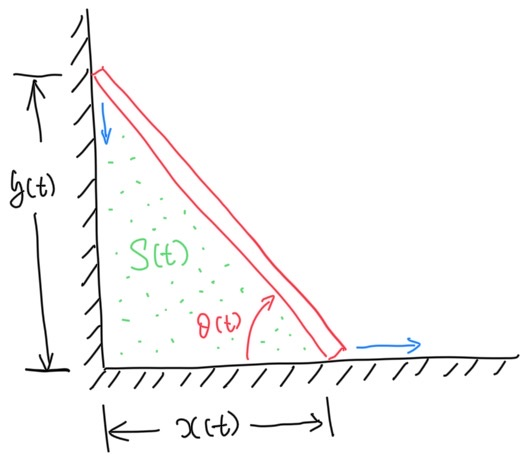
\includegraphics[width=5cm]{./images/ch2/ladder.jpg}
		\column{0.6\textwidth}
		(2)$S(t)=\df12x(t)y(t)$,故
		$$S'(t)=\df12[x'(t)y(t)+x(t)y'(t)],$$
		\pause 代入$x(t)=5,x'(t)=0.2,y(t)=\sqrt{11},y'(t)=-\df1{\sqrt{11}}$,
		可得所求三角形面积的变化速率为$-\df{7}{5\sqrt{11}}$m$^2$/s;
	\end{columns}
\end{frame}

\begin{frame}
	\linespread{1.5}
	\small 解:\it
	如图,
	\begin{columns}
		\column{0.4\textwidth}
		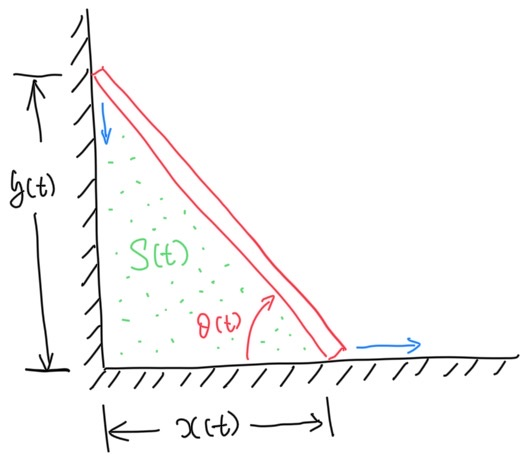
\includegraphics[width=5cm]{./images/ch2/ladder.jpg}
		\column{0.6\textwidth}
		(3)$\theta(t)=\arctan\df{y(t)}{x(t)}$,故
		$$\theta'(t)=\df1{1+\frac{y^2(t)}{x^2(t)}}
		=\df{y'(t)x(t)-y(t)x'(t)}{x^2(t)+y^2(t)},$$
		\pause 代入$x(t)=5,x'(t)=0.2,y(t)=\sqrt{11},y'(t)=-\df1{\sqrt{11}}$,
		可得指定时刻梯子和地面夹角的变化率为$-\df1{5\sqrt{11}}$弧度/s。\hfill$\Box$
	\end{columns}
\end{frame}

\begin{frame}
	\linespread{1.5}
	\ba{4.半径为$a$的圆球渐渐沉入盛有水的半径为$b(b>a)$的圆柱形容器中,若
	球的下降速度恒为$c$,求球浸没入水中恰好一半时,容器内水面上升的速率。
	}\pause
	
	\small 解:\it
	设$t$时刻,水中的球冠高度为$h(t)$,则此时水中的球冠体积
	$$V(t)=\df{\pi}3(3a-h(t))h^2(t),$$
	\pause 从而没入水中的球冠体积变换率
	$$V'(t)=\pi(2ah(t)-h^2(t))h'(t),$$
	\pause 相应地,桶内水面升高的速率为
	$$H'(t)=\df{V'(t)}{\pi [b^2-a^2+(a-h)^2]}
	=\df{2ah(t)-h^2(t)}{\pi [b^2-a^2+(a-h)^2]}h'(t),$$
	\pause 代入$h(t)=a,h'(t)=c$,即得所求水面上升的速率为$\df{a^2c}{b^2-a^2}$。
	\hfill$\Box$
\end{frame}

% !Mode:: "TeX:UTF-8"

\titlepage

\begin{frame}{说在前面}
	\linespread{1.5}
	  \begin{itemize}[<+-|alert@+>]
	    \item 过往的作业不订正、不补齐的不予批改,打分不超过\,\ba{C}
	    \item 不交作业的默认记为\,\ba{D}
	    \item 需要换作业本的,请“移植”照片,写清楚个人信息
	    \item 请自行完成SPOC课程中的测试
	    \item 第二次单元测试即将发布,成绩记入期末总成绩
	  \end{itemize}
\end{frame}

\begin{frame}{出现的问题}
	\linespread{1.5}
	  \begin{itemize}[<+-|alert@+>]
	    \item 用中值定理证明
	    \begin{itemize}
	      \item \it 写清楚理论依据:\b 由\ldots 定理 
	      \item \it 注意陈述的完整性:\b 存在$\xi\in(a,b)$
	      \item \it 注意语序:强烈建议不要从结果说起,写得像分析过程
	    \end{itemize}
	    \item 数学符号的书写
	    \begin{itemize}
	      \item \it 希腊字母:\b $\xi$像$\e$,$\eta$像$n$,$\mu$像$u$
	      \item \b\it $\ln 2$写成了$\ln^2$
	      \item \it 微分的表示:\b $1+\ln2\d x$和$(1+\ln2)\d x$不同!
	    \end{itemize}
	  \end{itemize}
\end{frame}

\section{2.6 微分}

\begin{frame}
	\linespread{1.5}
	\ba{1.设$y=x^3-2x$,
	\begin{enumerate}[(1)]
	  \setlength{\itemindent}{1cm}
	  \item 计算在$x=2$处当$\Delta x$分别为$1,\;0.1,\;
	  0.01$时的$\Delta y$和$\d y$;
	  \item 写出$x=2$时$y$的微分表达式。
	\end{enumerate}}
	\pause
	
% 	\bigskip
	
	\small 解:\it
	\begin{align*}
		\Delta y&=[(x+\Delta x)^3-2(x+\Delta x)]-(x^3-2x)\\
		&=(3x^2-2)\Delta x+3x\Delta x^2+\Delta x^3,\\
		\d y&=(3x^2-2)\d x=(3x^2-2)\Delta x.
	\end{align*}
\end{frame}

\begin{frame}
	\linespread{1.5}
	
	\small\it 当$x=2$时,
	\begin{align*}
		\Delta y|_{x=2}&
		=10\Delta x+6\Delta x^2+\Delta x^3,\\
		\d y|_{x=2}&=10\Delta x.
	\end{align*}
	\pause 进而
	\begin{enumerate}[(i)]
	  \item 当$x=2,\Delta x=1$时,$\Delta y=17,\;\d y=10$;
	  \item 当$x=2,\Delta x=0.1$时,$\Delta y=1.061,\;\d y=1$;
	  \item 当$x=2,\Delta x=0.01$时,$\Delta y=0.100601,\;\d y=0.1$。
	\end{enumerate}
	\hfill$\Box$
\end{frame}

\begin{frame}
	\linespread{1.5}
	\ba{2.已知$2^{xy}=x-y$,求$\d y|_{x=0}$。
	}\pause
	
	\bigskip
	
	\small 解:\it 
	已知方程两边求微分,可得
	$$2^{xy}\ln2(x\d y+y\d x)=\d x-\d y,$$
	进而
	$$\d y=\df{1-y2^{xy}\ln2}{1+x2^{xy}\ln2}\d x.$$
	\pause $x=0$时,$y=-1$,带入即得
	$$\d y|_{x=0}=(1+\ln2)\d x.$$
	\hfill$\Box$
\end{frame}

\begin{frame}
	\linespread{1.5}
	\ba{5.已知当$h\to 0$时,
	$$f(x+2h)-f(x)=h\sqrt{x^2+2x}+\circ(h),$$
	求$\d\left[f\left(\df1x\right)\right]$。}\pause

	\bigskip
	
	\small 解: \it 
	由已知
	$$\lim\limits_{h\to0}\df{f(x+2h)-f(x)}{2h}
	=\lim\limits_{h\to0}\df{h\sqrt{x^2+2x}+\circ(h)}{2h}
	=\df{\sqrt{x^2+2x}}2.
	$$
	也即$f'(x)=\df{\sqrt{x^2+2x}}2$,\pause 故
	$$\d\left[f\left(\df1x\right)\right]
	=f'\left(\df1x\right)\left(-\df1{x^2}\right)\d x
	=-\df{\sqrt{1+2x}}{2x^2|x|}\d x.$$
	\hfill$\Box$
\end{frame}

\begin{frame}
	\linespread{1.5}
	\ba{6.设$a>0$,$|x|<<a$(表示$|x|$远远小于$a$),证明近似公式
	$$\sqrt[n]{a^n+x}\approx a+\df{x}{na^{n-1}}.$$}\pause
	
	\bigskip
	
	\small 证:\it
	记$f(x)=\sqrt[n]{a^n+x}$,显然$f(0)=a$,
	又
	$$f'(x)=\df1n(a^n+x)^{\frac1n-1}\quad
	\Rightarrow f'(0)=\df1{na^{n-1}}.
	$$
	故由微分的几何意义,当$|x|<<a$时,总有
	$$\sqrt[n]{a^n+x}\approx f(0)+f'(0)x
	=a+\df{x}{na^{n-1}}.$$
	\hfill$\Box$
\end{frame}

\section{3.1 微分中值定理}

\begin{frame}
	\linespread{1.5}
	\ba{1.设$0<a<b$,$f(x)$在$[a,b]$上连续,在$(a,b)$内可导,证明:
	(1)$\exists\xi\in(a,b)$,使得:
	$f(b)-f(a)=\ln\df ba\cdot \xi f\,'(\xi)$}\pause
	
	\bigskip
	
	\small 证:\it
	注意到$f(x)$和$\ln x$在$[a,b]$上均连续,在
	在$(a,b)$内均可导,且$(\ln x)'=\df1x\ne 0$,故由Cauchy中值定理,
	存在$\xi\in(a,b)$,使得
	$$\df{f(b)-f(a)}{\ln b-\ln a}=\df{f'(\xi)}{\frac1{\xi}},$$
	整理后即证。\hfill$\Box$
\end{frame}

\begin{frame}
	\linespread{1.5}
	\ba{1.设$0<a<b$,$f(x)$在$[a,b]$上连续,在$(a,b)$内可导,证明:
	(2)$\exists\eta\in(a,b)$,使得:
    
    \centering $2\eta[f(b)-f(a)]=(b^2-a^2)f\,'(\eta)$
    
    }\pause
	
	\bigskip
	
	\small 证:\it
	注意到$f(x)$和$x^2$在$[a,b]$上均连续,在
	在$(a,b)$内均可导,且$(x^2)'=2x\ne 0$,故由Cauchy中值定理,
	存在$\eta\in(a,b)$,使得
	$$\df{f(b)-f(a)}{b^2-a^2}=\df{f'(\eta)}{2\eta},$$
	整理后即证。\hfill$\Box$
\end{frame}

\begin{frame}
	\linespread{1.5}
	\ba{1.设$0<a<b$,$f(x)$在$[a,b]$上连续,在$(a,b)$内可导,证明:
	(3)存在$x_1,x_2,x_3\in(a,b)$,使得
	
	\centering $f\,'(x_1)=(b+a)\df{f\,'(x_2)}{2x_2}=(a^2+ab+b^2)
	\df{f\,'(x_3)}{3x_3^2}$
    
    }\pause
	
	\bigskip
	
	\small 证:\it
	注意到$f(x)$和$x,x^2,x^3$在$[a,b]$上均连续,在
	在$(a,b)$内均可导,且$(x)'=x\ne 0,(x^2)'=2x\ne 0,
	(x^3)'=3x^2\ne 0$,故由Cauchy中值定理,
	存在$x_1,x_2,x_3\in(a,b)$,使得
	$$\df{f(b)-f(a)}{b-a}=f'(x_1),$$
	$$\df{f(b)-f(a)}{b^2-a^2}=\df{f'(x_2)}{2x_2}
	\quad\Rightarrow\quad
	\df{f(b)-f(a)}{b-a}=(b+a)\df{f'(x_2)}{2x_2},$$
	$$\df{f(b)-f(a)}{b^3-a^3}=\df{f'(x_3)}{3x_3^2}
	\quad\Rightarrow\quad
	\df{f(b)-f(a)}{b-a}=(a^2+ab+b^2)\df{f'(x_3)}{3x_3^2},$$
	整理后即证。\hfill$\Box$
\end{frame}

\begin{frame}
	\linespread{1.5}
	\ba{1.设$0<a<b$,$f(x)$在$[a,b]$上连续,在$(a,b)$内可导,证明:
	(4)若$f\,'(x)\ne 0$,则存在$\xi,\eta\in(a,b)$,使得
	
	\centering $\df{f'(\xi)}{f'(\eta)}=\df{e^b-e^a}{b-a}e^{-\eta}$
    
    }\pause
	
	\bigskip
	
	\small 证:\it
	由Lagrange和Cauchy中值定理,存在$\xi,\eta\in(a,b)$,使得
	$$\df{f(b)-f(a)}{b-a}=f'(\xi)
	\quad\Rightarrow\quad
	f(b)-f(a)=f'(\xi)(b-a).$$
	$$\df{f(b)-f(a)}{e^b-e^a}=\df{f'(\eta)}{e^{\eta}}
	\quad\Rightarrow\quad
	f(b)-f(a)=\df{e^b-e^a}{e^{\eta}}f'(\eta).$$
	整理后即证。\hfill$\Box$
\end{frame}

\begin{frame}
	\linespread{1.5}
	\ba{1.设$0<a<b$,$f(x)$在$[a,b]$上连续,在$(a,b)$内可导,证明:
	(5)存在$c\in(a,b)$,使得
	
	\centering $\df{1}{a-b}\left|\begin{array}{cc}
	a & b\\ f(a) & f(b)
	\end{array}\right|=f(c)-cf'(c).$
    
    }\pause
	
	\bigskip
	
	\small 证:\it
	由Cauchy中值定理,存在$c\in(a,b)$,使得
	\begin{align*}
		\df{1}{a-b}\left|\begin{array}{cc}
		a & b\\ f(a) & f(b)
		\end{array}\right|
		&=\df{af(b)-bf(a)}{a-b}=\df{\frac{f(b)}b-\df{f(a)}a}{\frac1b-\frac1a}\\
		&=\df{\left(\frac{f(x)}x\right)'_{x=c}}{\left(\frac1x\right)'_{x=c}}
		=f(c)-cf'c.
	\end{align*}
	即证。\hfill$\Box$
\end{frame}

\begin{frame}
	\linespread{1.5}
	\ba{1.设$0<a<b$,$f(x)$在$[a,b]$上连续,在$(a,b)$内可导,证明:
	(6)若$f(a)=0$,则存在$\mu\in(a,b)$,使得
	
	\centering $f'(\mu)=\df{a}{a+b-2\mu}f(\mu).$
    
    }\pause
	
	\bigskip
	
	\small 证:\it
	令$F(x)=f(x)\left(\df{a+b-2x}2\right)^{\frac a2}$,可以验证
	$F(x)$在$\left[a,\df{a+b}2\right]$上满足Rolle定理条件,故存在
	$\mu\in\left(a,\df{a+b}2\right)\subset(a,b)$,使得
	$$F'(\mu)=\left(\df{a+b-2\mu}2\right)^{\frac a2-1}
	\left[f'(\mu)\left(\df{a+b-2\mu}2\right)
	-f(\mu)a\right]=0,$$
	$\left(\df{a+b-2\mu}2\right)^{\frac a2-1}\ne0$,故必有
	$f'(\mu)\left(\df{a+b-2\mu}2\right)-f(\mu)\df a2=0,$
	即证。\hfill$\Box$
\end{frame}

\begin{frame}
	\linespread{1.5}
	\ba{2.$f(x)\in C^1[a,b]$,$f(a)=f(b)=0$,$f'_+(a)f'_-(b)>0$,
	证明:$f(x)$在$(a,b)$内至少有一个零点。}\pause
	
	\bigskip
	
	\small 证:\it
	不妨设$f'_+(a)>0,f'_-(b)<0$。由$f'_+(a)>0$可知,存在$\delta_1>0$,
	使对任意$x\in(a,a+\delta_1)$,总有
	$$\df{f(x)-f(a)}{x-a}>0\quad\Rightarrow
	\quad f(x)=f(x)-f(a)>0.$$
	因此可以取到某个$x_1\in(a,b)$,使得$f(x_1)>0$。
	
	\pause 类似地,由$f'_-(b)<0$,可知比存在某个$x_2\in(a,b)$,使得$f(x_2)<0$。
	
	\pause 至此,由介值定理,必存在某个$\xi$介于$x_1$和$x_2$之间,使得$f(\xi)=0$。
	\hfill$\Box$
\end{frame}

\begin{frame}
	\linespread{1.5}
	\ba{3.证明:对任意$x>1$,
	
	\centering $(x^2-1)\ln x\geq(x-1)^2$。
	
	}\pause
	
	\bigskip
	
	\small 证:\it
	由Lagrange中值定理,存在$\xi$介于$x$和$1$之间,使得
	$$\df{\ln x-\ln 1}{x-1}=\df1{\xi},$$
	\pause 显然$0<\xi<x+1\Rightarrow\df1{\xi}>\df1{x+1}$,带入前式整理后即证。
	\hfill$\Box$
\end{frame}

\begin{frame}
	\linespread{1.5}
	\ba{4.$e<a<b<e^2$,证明:$\ln^2b-\ln^2a>\df2{e^2}(b-a)$。}\pause
	
	\bigskip
	
	\small 证:\it
	由Lagrange中值定理,存在$\xi\in(a,b)$,使得
	$$\df{\ln^2b-\ln^2a}{b-a}=\df{2\ln\xi}{\xi},$$
	注意到$e<\xi<e^2$,故
	$$1<\ln\xi<2,\quad \xi<e^2,$$
	故
	$\df{2\ln\xi}{\xi}>\df2{e^2},$
	代入前式整理即证。
	\hfill$\Box$
\end{frame}

\begin{frame}
	\linespread{1.5}
	\ba{5.$f(x)$在$x>0$二阶可导,$f''(x)>0$,令$u_n=f(n)\;
	 (n\in\mathbb{Z}_+)$,证明:若$u_1<u_2$,则$\{u_n\}$必发散;
	问:若$u_1>u_2$,$\{u_n\}$是否必收敛?(若正确,证明之;否则给出反例。)}\pause
	
	\bigskip
	
	\small 证:\it
	由$f''(x)>0$可知,$f'(x)$单调递增。若$u_1<u_2$,也即$f(1)<f(2)$,
	由Lagrange中值定理,存在$\xi_1\in(1,2)$,使得
	$$0<\df{f(2)-f(1)}{2-1}=f'(\xi_1),$$
	进而可知对任意$x>2$,均有$f'(x)>f'(\xi_1)$。
\end{frame}

\begin{frame}
	\linespread{1.5}
% 	\ba{5.$f(x)$在$x>0$二阶可导,$f''(x)>0$,令$u_n=f(n)\;
% 	 (n\in\mathbb{Z}_+)$,证明:若$u_1<u_2$,则$\{u_n\}$必发散;
% 	问:若$u_1>u_2$,$\{u_n\}$是否必收敛?(若正确,证明之;否则给出反例。)}\pause
	
% 	\bigskip
	
	\small \it
	对任意$n\geq2$,由Lagrange中值定理,存在$\xi_n\in(n,n+1)$,使得
	$$\df{f(n+1)-f(n)}{(n+1)-n}=f'(\xi_n)>f'(\xi_1)$$
	进而可得
	$$
	f(n+1)>f(n)+f'(\xi_1)>f(n-1)+2f'(\xi_1)>\ldots>f(1)+nf'(\xi_1),
	$$
	由此显然可知$\{u_n\}$发散。
	
	若$u_1>u_2$,$\{u_n\}$未必收敛。例如:$f(x)=(x-3)^2$,其中$u_1=4>1=u_2$,
	但显然$\{(n-3)^2\}$发散。\hfill$\Box$
\end{frame}

%   % !Mode:: "TeX:UTF-8"

\begin{frame}
	\frametitle{常微分方程习题课}
	\linespread{1.5}
	  \begin{itemize}
% 	    \item 理解微分方程及其相关概念
	    \item 一阶微分方程解法与常用解题技巧
	    \item 两类可降阶的二阶方程的解法及其高阶推广
	    \item 二阶线性微分方程解的结构
	    \item 解二阶常系数齐次线性微分方程的特征方程法及其高阶推广
	    \item 解两类二阶常系数非齐次线性微分方程的待定系数法
	  \end{itemize}
\end{frame}

\section{问题讨论}

\begin{frame}{问题讨论}
	\linespread{1.5}
	\alert{问:}已知$n$阶线性微分方程的$n$个解,
	能否写出这个微分方程及其通解?\pause\\[1ex]
	
	\alert{答:}{\it 不一定!}\pause {\it 除非 
	这$n$个解恰好线性无关。} \pause 
	
	\bigskip
	\alert{问:}适当确定微分方程通解中的参数值,可以得到其任意的特解?\pause \\[1ex]
	
	\alert{答:}{\it 错!}\pause 反例:{\it $y'=\sin x\cos^2y$}.
\end{frame}

\begin{frame}{问题讨论}
	\linespread{1.2}
	\alert{问:}$y_1=(x-1)^2$和$y_2=(x+1)^2$都是方程
	$$(x-1)^2y''-2xy'+2y=0,$$
	和
	$$2yy''-(y')^2=0$$
	的解。但二者的线性组合
	$$y=C_1(x-1)^2+C_2(x+1)^2,\;(C_1,C_2\in\mathbb{R})$$
	却仅能满足前一个方程,为什么?\pause 
	
	\alert{答:}{\it 第二个方程不是线性方程!}
\end{frame}

\section{补充例题}

\begin{frame}{填空}
	\linespread{2}
	\ba{1.}\;$y''+4y'+4y=1$的通解为
	\underline{\uncover<2->{\;\b{$(C_1+C_2x)e^{-2x}+1/4$}}\;}.\\[1em]
	
	\ba{2.}\;设$e^x(C_1\cos x+C_2\sin x)$为首项系数为$1$的某二阶常系数
	齐次线性微分方程的通解,则该微分方程为
	\underline{\uncover<3->{\;\b{$y''-2y'+2y=0$}}\;}.\\[1em]
	
	\ba{3.}\;设$\cos x$与$xe^x$分别为某$n$阶常系数齐次线性微分方程的两个解,
	则最小的$n=$\underline{\uncover<4->{\;\b{$4$}}\;},相应的首项
	系数为$1$的方程为\underline{\uncover<5->{\;\b{$
	y^{(4)}-2y^{(3)}+2y''-2y'+y=0$}\;}}
	
% 	方程$xy''-2xy'+2y=x\ln x$的通解为
% 	为\underline{\uncover<6->{\;\b{$
% 	C_1x+C_2x^2-\left(\df12\ln^2x+\ln x\right)x$}\;}}
\end{frame}

\begin{frame}{选择}
	\linespread{1.5}
	\ba{1.}\;方程$y''+4y=e^{3x}+x\sin 2x$的一个特解形式是
	(\underline{\uncover<2->{\;\b{A}}\;})
	\begin{enumerate}[(A)]
	  \item $Ae^{3x}+x[(Bx+C)\cos2x+(Dx+E)\sin2x]$
	  \item $Ae^{3x}+(Bx+C)\cos2x+(Dx+E)\sin2x$
	  \item $Axe^{3x}+x[(Bx+C)\cos2x+(Dx+E)\sin2x]$
	  \item $Axe^{3x}+(Bx+C)\cos2x+(Dx+E)\sin2x$
	\end{enumerate}
\end{frame}

\begin{frame}{选择}
	\linespread{1.3}
	\ba{2.}\;设$y_1(x),y_2(x),y_3(x)$为方程
	$$y''+p(x)y'+q(x)y=f(x)$$
	的三个线性无关的解,$C_1,C_2$为任意常数,则该非齐次线性微分方程的通解为
	(\underline{\uncover<2->{\;\b{C}}\;})
	\begin{enumerate}[(A)]
	  \item $(C_1+C_2)y_1+(C_2-C_1)y_2+(1-C_2)y_3$
	  \item $(C_1+C_2)y_1+(C_2-C_1)y_2+(C_1-C_2)y_3$
	  \item $C_1y_1+(C_2-C_1)y_2+(1-C_2)y_3$
	  \item $C_1y_1+(C_2-C_1)y_2+(C_1-C_2)y_3$
	\end{enumerate}
\end{frame}

\begin{frame}{选择}
	\linespread{1.3}
	\ba{3.}\;设$y=f(x)$为方程$y''-2y'+4y=0$
	的一个解,若$f(x_0)>0,f'(x_0)=0$,
	则函数$f(x)$在$x_0$
	(\underline{\uncover<2->{\;\b{A}}\;})
	\begin{enumerate}[(A)]
	  \item 取极大值
	  \item 取极小值
	  \item 的某个领域内单调增加
	  \item 的某个领域内单调减少
	\end{enumerate}
\end{frame}

\begin{frame}{选择}
	\linespread{1.3}
	\ba{4.}\;设$y(x)$为方程$y''+py'+qy=e^{3x}$满足初始条件$y(0)=y'(0)=0$
	的解,则$\limx{0}\df{\ln(1+x^2)}{y(x)}$
	(\underline{\uncover<2->{\;\b{C}}\;})
	\begin{enumerate}[(A)]
	  \item 不存在
	  \item 等于$1$
	  \item 等于$2$
	  \item 等于$3$
	\end{enumerate}
\end{frame}

\begin{frame}{选择}
	\linespread{1.3}
	\ba{5.}\;设$y(x)$满足$x\d y+(x-2y)\d x=0$,且曲线$y=y(x)$与直线$x=1$
	及$x$轴所围平面图形绕$x$轴旋转所得旋转体的体积最小,则$y(x)=$
	(\underline{\uncover<2->{\;\b{C}}\;})
	\begin{enumerate}[(A)]
	  \item $x-\df14x^2$
	  \item $x+\df54x^2$
	  \item $x-\df54x^2$
	  \item $x+\df14x^2$
	\end{enumerate}
\end{frame}

\begin{frame}{选择}
	\linespread{1.3}
	\ba{6.}\;方程$y''+by'+y=0$的每个解都在$x>0$上有界,则实数$b$的取值范围是
	(\underline{\uncover<2->{\;\b{A}}\;})
	\begin{enumerate}[(A)]
	  \item $[0,+\infty)$
	  \item $(-\infty,0]$
	  \item $(-\infty,4]$
	  \item $(-\infty,+\infty]$
	\end{enumerate}
\end{frame}

% \begin{frame}{解方程}
% 	\linespread{1.5}
% 	\begin{enumerate}
% 	  \item $xy'\ln x+y=\ln x$.\hfill \b$t=\ln x$
% 	\end{enumerate}
% \end{frame}

\begin{frame}{解答题}
	\linespread{1.2}
	\ba{1.}\;设$f(x)$为连续函数,且
	$$f(x)=e^{-x}+\dint_0^xf(t)\d t,$$
	求$f(x)$.
	
	\pause\alert{提示:}\it\b  积分方程通常自带初值条件$f(0)=1$.\pause
	$$f'(x)-f(x)=-e^{-x}\quad\Rightarrow\quad 
	f(x)=\df12(e^x+e^{-x}).$$
	
	\pause 不带初值条件的例子:\ba{习题7.2-8}
\end{frame}

\begin{frame}{解答题}
	\linespread{1.2}
	\ba{2.}\;设$f(x)$为连续函数,且
	$$f(x)=e^{2x}+\dint_0^xtf(x-t)\d t,$$
	求$f(x)$.
	
	\pause\alert{提示:}\it\b $f(0)=1,f'(0)=2$\pause  
	$$f''(x)-f(x)=4e^{2x}\quad\Rightarrow\quad 
	f(x)=-\df12e^x+\df16e^{-x}+\df43e^{2x}.$$
\end{frame}

% \begin{frame}{解答题}
% 	\linespread{1.2}
% 	\ba{3.(习题7.3-7)}函数$y(x)\;(x\geq 0)$二阶可导,$y'(x)>0$,
% 	$y(0)=1$,过其上任一点$(x,y)$作曲线的切线和至$x$轴的垂线,该两直线
% 	与$x$轴所围成的三角形面积记为$S_1(x)$,又区间$[0,\alert{x}]$
% 	(\alert{\it 此处教材印刷错误!})上以$y(x)$为曲边
% 	的曲边梯形面积记为$S_2(x)$。已知$2S_1-S_2=1$,求$y(x)$。
% 	
% 	\pause\alert{提示:}\it\b   
% 	$$\df{y^2}{y'}-\dint_0^xy(t)\d t=1\quad\Rightarrow\quad 
% 	yy''=(y')^2,\;y'(0)=1.$$
% 	\pause 结合$y(0)=1$,解得$y=e^x$.
% \end{frame}

\begin{frame}{解答题}
	\linespread{1.2}
	\ba{3.}\;设对任意$x,y\in\mathbb{R}$
	$$f(x+y)=f(x)e^y+f(y)e^x,$$
	$f'(0)=a\ne 0$,求$f(x)$.
	
	\pause\alert{提示:}\it\b 必须用定义计算$f'(x)$,
	$$\lim\limits_{\Delta x\to 0}\df{f(x+\Delta x)-f(x)}{\Delta x}
	=f(x)+ae^x.$$
	\pause 类似题目:\alert{\bf 习题7.2-7,辅导书(下)-P256-例5}
\end{frame}

\begin{frame}{解答题}
	\linespread{1.2}
	\ba{4.}\;某同学将乘积的导数公式错误地记作$(fg)'=f'g'$,然而在一次求导时
	居然得到了正确的结果。目前知道他使用的$f(x)=e^{x^2},(x>1/2)$,
	问他用到的$g(x)$可能是什么?
	
	\pause\alert{提示:}\it\b  
	$$\left(e^{x^2}g\right)'=\left(e^{x^2}\right)'g'$$
	从而$(2x-1)g'=2xg$,解得
	$$g=Ce^x\sqrt{2x-1}$$
\end{frame}

\begin{frame}{解答题}
	\linespread{1.5}
	\ba{5.}\;设二阶常系数线性微分方程
	$$y''+\alpha y'+\beta y=\gamma e^x$$
	的一个解为$y=e^{2x}+(1+x)e^x$,试确定其中的常数$\alpha,\beta,\gamma$.
	
	\pause\alert{提示:}\it\b $\alpha=-3,\beta=2,\gamma=-1$.
\end{frame}

\begin{frame}{解答题}
	\linespread{1.2}
	\ba{6.}\;求方程$y''+2y'+2y=2e^{-x}\cos^2\df x2$的通解.
	
	\pause\alert{提示:}\it\b 
	$$2e^{-x}\cos^2\df x2=e^{-x}+e^{-x}\cos x,$$
	利用叠加原理分别求解两个常系数非齐次线性微分方程。
\end{frame}

% \begin{frame}{解答题}
% 	\linespread{1.2}
% 	\alert{(2003考研)} 设$y(x)$在$\mathbb{R}$上具有二阶连续导数,
% 	$y'\ne 0$,$x=x(y)$为其反函数。
% 	\begin{enumerate}
% 	  \item 试将$x=x(y)$所满足的微分方程
% 	  $$\df{\d^2x}{\d y^2}+(y+\sin x)\left(\df{\d x}{\d y}\right)^3=0$$
% 	  变换为$y=y(x)$所满足的微分方程;
% 	  \item 求变换后的微分方程满足初始条件$y(0)=0$和$y'(0)=1.5$的解。
% 	\end{enumerate}
% 	
% 	\pause\alert{提示:}\it\b 
% 	$y''-y=\sin x\quad\Rightarrow\quad y=e^x-e^{-x}-\df12\sin x $
% \end{frame}

\begin{frame}{应用题}
	\linespread{1.2}
	\ba{7.}\;令$t=\tan x$,将方程
	$$\cos^4xy''_{xx}+2\cos^2x(1-\sin x\cos x)y'_x+y=e^{-\tan x}$$
	变换为$y$关于$t$的微分方程,并求其通解。
	
	\pause\alert{提示:}\it\b 
	$$y''_{tt}+2y'_t+y=e^{-t}$$
	$$y=\left(C_1+C_2\tan x+\df12\tan^2x\right)e^{-\tan x}$$
\end{frame}

\section{微分方程的应用}

\begin{frame}{应用题}
	\linespread{1.4}
	\ba{8.}\;已知某凹曲线任一点处的曲率为$\df1{2y^2\cos\alpha}$,其中
	$\alpha$为该点处的切线倾角($\cos\alpha>0$),且曲线在
	点$(1,1)$处的切线是水平的,求该曲线的方程。
	
	\pause\alert{提示:}\it\b $\cos\alpha>0=\df1{\sqrt{1+(y')^2}},
	\;y''>0$
	$$2y^2y''=[1+(y')^2]^2\quad\Rightarrow\quad
	4y=(x-1)^2+4$$
\end{frame}

% \begin{frame}{应用题}
% 	\linespread{1.2}
% 	\ba{(习题7.4-14)}一根挂在钉子上的链条,最初两端距离钉子
% 	分别为$8$m和$12$m,如不计钉子
% 	对链条产生的摩擦力,求链条从钉子上完全滑落所需的时间。
% 	
% 	\pause\alert{提示:}\it\b 设$x$为较长一端端点据钉子的距离
% 	$$\left\{\begin{array}{l}
% 		x''-\df g{10}x=-g\\
% 		x(0)=12\\
% 		x'(0)=0
% 	\end{array}\right.$$
% % 	\pause
% % 	\alert{思考:}若摩擦力等于$1$m长的链条的重量,模型又是怎样的?
% \end{frame}

\begin{frame}{应用题}
	\linespread{1.2}
	\ba{9.}\;已知某车间容积$V$,其空气中CO$_2$的密度为$\rho_1$,现以CO$_2$浓度$\rho_2(<<\rho_1)$的
	新鲜空气输入,问每分钟应输入多少才能在$T$分钟后使车间中CO$_2$的含量不超过$\rho_0$。
	(注:假设新注入的空气能够与原有空气立即混合达到均匀,且空气不会被压缩。)

	\pause\alert{提示:}\it\b 设$t$分钟时的$CO_2$含量为$C(t)$,
	$$C'=\rho_2V_1-C\df{V_1}{V},C(0)=\rho_1V$$
\end{frame}

\begin{frame}{应用题}
	\linespread{1.2}
	\ba{10.}\;某湖泊的水量为$V$,每年排入湖内的污水和净水量均为$V/6$,且湖内的总水量不变。
	已知1999年底湖内的污染物含量为$5m_0$。为了治理污染,从2000初开始,限定排入
	湖中的污水中污染物浓度不得超过$m_0/V$。问至少需要经过多少年,
	湖内的污染物含量能够降至$m_0$以下?(注:假设湖水中的污染物浓度时均匀分布的。)

	\pause\alert{提示:}\it\b 
	$$m'=\df{m_0}6-\df m3,\quad m=\df{m_0}2(1+9e^{-t/3})$$
	$t=6\ln3$年后,达到要求。
\end{frame} %常微分方程习题课
% 	\begin{frame}{向量的运算、空间平面与直线}
	\linespread{1.2}
	\begin{enumerate}
	  \item 内积(投影)、外积(面积)、混合积(体积,三线共面)
	  \item 平面方程中的几何特征
	  \item 不同直线方程间的相互转换
	  \item 空间几何问题的一题多解
	\end{enumerate}
\end{frame}

\begin{frame}{判断}
	\linespread{1.2}
	\begin{enumerate}
	  \item $\bm{a}\cdot\bm{a}\cdot\bm{a}=\bm{a}^3$\quad\pause\ba{$\times$}\pause
	  \item $\bm{a}\ne 0$时,$\df{\bm{a}}{\bm{a}}=1$\quad\pause\ba{$\times$}\pause
	  \item $\bm{a}(\bm{a}\cdot\bm{b})=\bm{a}^2\bm{b}$
	    \quad\pause\ba{$\times$}\pause
	  \item $(\bm{a}\cdot\bm{b})^2=\bm{a}^2\bm{b}^2$\quad\pause\ba{$\times$}\pause
	  \item $|\bm{a}\cdot\bm{b}|=|\bm{a}|\cdot|\bm{b}|$
		\quad\pause\ba{$\times$}\pause
	  \item $(\bm{a}+\bm{b})\times(\bm{a}-\bm{b})=\bm{a}\times\bm{a}
  		-\bm{b}\times\bm{b}=0$
  		\quad\pause\ba{$\times$}\pause
  	  \item $\bm{a}\ne 0$时,$\bm{a}\cdot\bm{b}
  	  	=\bm{a}\cdot\bm{c}\Rightarrow\bm{b}=\bm{c}$
  	  	\quad\pause\ba{$\times$}\pause
  	  \item  $\bm{a}\ne 0$时,$\bm{a}\times\bm{b}
  	  	=\bm{a}\times\bm{c}\Rightarrow\bm{b}=\bm{c}$
  	  	\quad\pause\ba{$\times$}
	\end{enumerate}
\end{frame}

\begin{frame}{填空}
	\linespread{1.2}
	\ba{1.}\;设$(\bm{a}\times\bm{b})\bm{c}=2$,则
	$[(\bm{a}+\bm{b})\times(\bm{b}+\bm{c})](\bm{c}+\bm{a})=$
	\underline{\uncover<2->{\;\b{$4$}}\;}.\\[1em]
	
	\ba{2.}\;设$\bm{a},\bm{b}$均为非零向量,则
	其角平分线上的向量为
	\underline{\uncover<3->{\;\b{$C\left(\df{\bm{a}}{|\bm{a}|}
	+\df{\bm{b}}{|\bm{b}|}\right),\;(C\in\mathbb{R})$}}\;}.\\[1em]
	
	\ba{3.}\;设$\bm{a},\bm{b},\bm{c}$均为非零向量,且$\bm{a}=\bm{b}\times\bm{c}$,
	$\bm{b}=\bm{c}\times\bm{a}$,
	$\bm{c}=\bm{a}\times\bm{b}$则
	$|\bm{a}|+|\bm{b}|+|\bm{c}|=$
	\underline{\uncover<4->{\;\b{$3$}}\;}.\\[1em]
\end{frame}

\begin{frame}{填空}
	\linespread{1.2}
	\ba{4.}\;设$|\bm{a}|=2,|\bm{b}|=2$,$\bm{a}$和$\bm{b}$
	的夹角为$\pi/3$,则$|2\bm{a}-3\bm{b}|=$
	\underline{\uncover<2->{\;\b{$2\sqrt7$}}\;}.\\[1em]
	
	\ba{5.}\;设$\bm{a},\bm{b}$均为非零向量,且$|\bm{b}|=1$,$\bm{a}$和$\bm{b}$
	的夹角为$\pi/4$,则$\limx{0}\df{|\bm{a}+x\bm{b}|-|\bm{a}|}{x}=$
	\underline{\uncover<3->{\;\b{$\df{\sqrt2}2$}}\;}.\\[1em]
	
	\ba{6.}\;平面$Ax+By+Cz+D_i=0\;(i=1,2)$之间的距离为
	\underline{\uncover<4->{\;\b{$\df{|D_1-D_2|}{\sqrt{A^2+B^2+C^2}}$}}\;}.
\end{frame}

\begin{frame}{选择}
	\linespread{1.3}
	\ba{1.}\;设$\bm{a},\bm{b},\bm{c}$均为非零向量,则与$\bm{a}$不垂直的是
	(\underline{\uncover<2->{\;\b{D}}\;})
	\begin{enumerate}[(A)]
	  \item $(\bm{a}\cdot\bm{c})\bm{b}-(\bm{a}\cdot\bm{b})\bm{c}$
	  \item $\bm{b}-\left(\df{\bm{a}\cdot\bm{b}}{\bm{|a|}^2}\right)\bm{a}$
	  \item $\bm{a}\times\bm{b}$
	  \item $\bm{a}+(\bm{a}\times\bm{b})\times\bm{a}$
	\end{enumerate}
\end{frame}

\begin{frame}{选择}
	\linespread{1.3}
	\ba{2.}\;设$\bm{a},\bm{b}$为非零向量,$|\bm{a}-\bm{b}|=|\bm{a}+\bm{b}|$,则
	(\underline{\uncover<2->{\;\b{C}}\;})
	\begin{enumerate}[(A)]
	  \item $\bm{a}-\bm{b}=\bm{a}+\bm{b}$
	  \item $\bm{a}=\bm{b}$
	  \item $\bm{a}\cdot\bm{b}=0$
	  \item $\bm{a}\times\bm{b}=0$
	\end{enumerate}
\end{frame}

\begin{frame}{选择}
	\linespread{1.3}
	\ba{3.}\;设$\bm{a},\bm{b}$为非零向量,且满足
	$(\bm{a}+3\bm{b})\perp(7\bm{a}-5\bm{b})$,
	$(\bm{a}-4\bm{b})\perp(7\bm{a}+2\bm{b})$,则
	向量$\bm{a}$和$\bm{b}$的夹角为
	(\underline{\uncover<2->{\;\b{C}}\;})
	\begin{enumerate}[(A)]
	  \item $0$
	  \item $\pi/2$
	  \item $\pi/3$
	  \item $2\pi/3$
	\end{enumerate}
\end{frame}

\begin{frame}{选择}
	\linespread{1.3}
	\ba{4.}\;设平面$\pi$位于平面$x-2y+z-2=0$和$x-2y+z-6=0$之间,
	且与此二平面的距离之比为$1:3$,则$\pi$的方程为
	(\underline{\uncover<2->{\;\b{A}}\;})
	\begin{enumerate}[(A)]
	  \item $x-2y+z-5=0$或$x-2y+z-3=0$
	  \item $x-2y+z+8=0$
	  \item $x+2y+4z=0$
	  \item $x-2y+5z-3=0$
	\end{enumerate}
\end{frame}

\begin{frame}{选择}
	\linespread{1.3}
	\ba{5.}\;设$\left|\begin{array}{ccc}
	a_1 & b_1 & c_1\\ a_2 & b_2 & c_2\\ a_3 & b_3 & c_3
	\end{array}\right|\ne 0$,则
	直线
	$\df{x-a_3}{a_1-a_2}=\df{y-b_3}{b_1-b_2}$
	$=\df{z-c_3}{c_1-c_2}$
	和
	$\df{x-a_1}{a_2-a_3}=\df{y-b_1}{b_2-b_3}=\df{z-c_1}{c_2-c_3}$
	(\underline{\uncover<2->{\;\b{A}}\;})
	\begin{enumerate}[(A)]
	  \item 相交于一点
	  \item 重合
	  \item 平行但不重合
	  \item 异面直线
	\end{enumerate}
\end{frame}

\begin{frame}{解答}
	\linespread{1.2}
	\ba{1.}\;过原点且与
	$$\left\{\begin{array}{l}
	x=1\\ y=-1+t\\ z=2+t
	\end{array}\right.$$
	和$x+1=\df{y+2}2=z-1$都平行的平面方程。
	
	\pause\alert{提示:}\it\b  
	$$x-y+z=0$$
\end{frame}

\begin{frame}{解答}
	\linespread{1.2}
	\ba{2.}\;求过点$M(3,1,-2)$和直线$\df{x-4}5=\df{y+3}2=\df z1$
	的平面方程。
	
	\pause\ba{法一:}\it\b  
	$\bm{n}=\bm{s}\times\bm{MM_1}=(-8,9,22)$,平面方程
	$$8x-9y-22x-59=0$$
	
	\pause\ba{法二:}
	直线的一般式方程:$\left\{\begin{array}{l}x-5y-4=0\\ 
	y-2z+3=0\end{array}\right.$,进而可得$\lambda=8,\mu=-9$
\end{frame}

\begin{frame}
	\linespread{1.2}
	\ba{3.}\;过直线
	$\df{x-1}2=\df{y+2}{-3}=\df{z-2}2$且垂直于平面
	$3x+2y-z=5$的平面方程。
	
	\pause\alert{提示:}{\b  
	$$x-8y-13z+9=0$$}
	
	\pause
	\ba{4.}\;求过直线
	$$\left\{\begin{array}{l}
		x+5y+z=0\\
		x-z+4=0
	\end{array}\right.$$
	且与平面$\pi:x-4y-8z+12=0$的夹角为$\pi/4$的平面方程。
\end{frame}

\begin{frame}
	\linespread{1.2}
	\ba{5.}\;过点$(-1,0,4)$,平行于平面
	$3x-4y+z=10$,且与直线$x+1=y-3=\df z2$
	相交的直线方程。

	\pause\alert{提示:}\it\b
	$$\df{x+1}{16}=\df{y}{19}=\df{z-4}{28}$$
\end{frame}

\begin{frame}
	\linespread{1.2}
	\ba{6.}\;已知$P(3,1,-4)$和$L:\df{x+1}2=\df{y-4}{-2}=z-1$,求
	\begin{enumerate}
	  \item $P$到$L$的距离;
	  \item $P$在$L$上的垂足$Q$的坐标;
	  \item 设$R(1,2,3)$在$L$上的垂足为$N$,求$QN$的长度。
	\end{enumerate}
	
	\pause\alert{提示:}\it\b
	$(1)\sqrt{41}$\quad$(2)(1,2,2)$\quad$(3)\df13$  
\end{frame}

\begin{frame}
	\linespread{1.2}
	\ba{7.}\;已知直线
	$$L_1:\left\{\begin{array}{l}
		x+y+z+1=0\\
		2x-y+3z+4=0
	\end{array}\right.
	\quad
	L_2:\left\{\begin{array}{l}
		x=-1+2t\\
		y=-t\quad(t\in\mathbb{R})\\
		z=2-2t
	\end{array}\right.
	$$
	\begin{enumerate}[(1)]
% 	  \setlength{\itemindent}{1cm}
	  \item 证明两直线异面;
	  \item 求两直线间的距离;
	  \item 求二者的公垂线方程。
	\end{enumerate}
	
	\pause\alert{提示:}\it\b
	$L_1,L_2$的标准式方程
	$$\df{x+3}4=\df{y-1}{-1}=\df{z-1}{-3},\quad
	\df{x+1}2=\df y{-1}=\df{z-2}{-2}$$
\end{frame}

\begin{frame}
	\linespread{1.2}
	\ba{8.}\;计算由以下平面所围成的立体体积:
	$$a_ix+b_iy+c_iz=\pm h_i,\;i=1,2,3,$$
	其中:$a_i,b_i,c_i$为常数,$h_i\ne0(i=1,2,3)$,且
	$$\Delta=\left|\begin{array}{ccc}
	a_1 & b_1 & c_1\\ a_2 & b_2 & c_2 \\ a_3 & b_3 & c_3
	\end{array}\right|\ne 0$$
	
	\pause\alert{提示:}\b
	$$\left[(\bm{s}_1\times\bm{s}_2)\times
	(\bm{s}_2\times\bm{s}_3)\right]\cdot(\bm{s}_3\times\bm{s}_1)=
	\left[(\bm{s}_1\times\bm{s}_2)\cdot\bm{s}_3\right]^2$$ 
\end{frame}

\begin{frame}{讨论}
	\linespread{1.2}
	\begin{enumerate}
	  \item 证明:$\bm{s}_1\times(\bm{s}_2\times\bm{s}_3)
	  	=(\bm{s}_1\cdot\bm{s}_3)\bm{s}_2
		-(\bm{s}_1\cdot\bm{s}_2)\bm{s}_3$\pause
	  \item 证明:$\left[(\bm{s}_1\times\bm{s}_2)\times
	  	(\bm{s}_2\times\bm{s}_3)\right]
		\cdot(\bm{s}_3\times\bm{s}_1)
		=\left[(\bm{s}_1\times\bm{s}_2)\cdot\bm{s}_3\right]^2$\pause
	  \item $\bm{s}_1\times(\bm{s}_2\times\bm{s}_3)
	  =(\bm{s}_1\times\bm{s}_2)\times\bm{s}_3$成立吗?
	\end{enumerate}
	\ba{提示:}\it\b 反例:
	$$\bm{j}\times(\bm{i}\times\bm{i})=0$$
	$$(\bm{j}\times\bm{i})\times\bm{i}=-\bm{k}\times\bm{i}=-\bm{j}$$
\end{frame} %空间直线与平面习题课
% 	\renewcommand{\b}{\color{blue!80!black}}

\begin{frame}{曲线积分与曲面积分}
	\linespread{1.2}
	\begin{enumerate}
	  \item 曲线和曲面积分的计算
	  \begin{itemize}
	    \item {\it 第一型:方向无关,第二型:方向敏感}
	    \item {\it 第一型:质量类应用;第二型:向量场类应用}
	  \end{itemize}
	  \item Green公式和Gauss公式
	  {\it
	  \begin{itemize}
	    \item Green公式的证明
	    \item “补全”和“挖洞”
	    \item 全微分与原函数(势函数)
	    \item 散度、旋度、无源场、无旋场、保守场、C-R条件
	  \end{itemize}
	  }
	  \item 对称性在各种积分中的应用
	  \item 不同类型积分之间的相互转换
	\end{enumerate}
\end{frame}

\begin{frame}{填空}
	\linespread{1.5}
% 	$\star$
	\ba{1、}设$L$为曲线$x=\df{3at}{1+t^3},y=\df{3at^2}{1+t^3}$上$t$由
	$0$到$+\infty$的一段,$a>0$,则$\dint_Lx\d y-y\d x=$
	\underline{\uncover<2->{\;\b{$3a^2$}}\;}.\\[1em]
	
% 	\pause\pause
	\ba{2、}$f(x)$连续可导,$L$为$(3,2/3)$到$(1,2)$的直线,
	则$\dint_L\df{1+y^2f(xy)}y\d x+\df x{y^2}[y^2f(xy)-1]\d y=$
	\underline{\uncover<3->{\;\b{$-4$}}\;}.\\[1em]
	
% 	\pause\pause
	\ba{3、}$\ds\iint\limits_{z=\sqrt{a^2-x^2-y^2}}(x+y+z)\d S=$
	\underline{\uncover<4->{\;\b{$\pi a^3$}}\;}.\\[1em]
\end{frame}

\begin{frame}
	\linespread{1.5}
% 	$\star$
	\ba{4、}设$\Sigma$为平面$x+y+z=1$在第一卦限的上侧,$f(x,y,z)$连续,则
	$\ds\iint\limits_{\Sigma}[f(x,y,z)+x]\d y\d z-[2f(x,y,z)-y]\d z\d x+
	[f(x,y,z)+z]\d x\d y=$
	\underline{\uncover<2->{\;\b{$\df12$}}\;}.\\[1em]
	
% 	\pause\pause
	\ba{5、}设$\Sigma$为锥面$z=\sqrt{x^2+y^2}(0\leq z\leq 1)$的下侧,则
	$\ds\iint\limits_{\Sigma}x\d y\d z+2y\d z\d x+3(z-1)\d x\d y=$
	\underline{\uncover<3->{\;\b{$2\pi$}}\;}.\\[1em]
	
% 	\pause\pause
	\ba{6、}设$L$是摆线$x=t-\sin t-\pi,y=1-\cos t$从$t=0$
	到$t=2\pi$的一段,则$\dint_L\df{(x-y)\d x+(x+y)\d y}{x^2+y^2}=$
	\underline{\uncover<4->{\;\b{$-\pi$}}\;}.\\[1em]
\end{frame}

\begin{frame}{选择}
	\linespread{1.5}
	\ba{1、}设$\Gamma$为上半圆周$x^2+y^2=2x$从原点到$(1,1)$的部分,则
  	$\dint_{\Gamma}P(x,y)\d x+Q(x,y)\d y=$
	(\underline{\uncover<2->{\;\b{C}}\;})
	\begin{enumerate}[(A)]
	  \item $\dint_{\Gamma}\left[P(x,y)(x-1)+Q(x,y)\sqrt{2x-x^2}\right]\d s$
      \item $\dint_{\Gamma}\left[P(x,y)(1-x)-Q(x,y)\sqrt{2x-x^2}\right]\d s$
      \item $\dint_{\Gamma}\left[P(x,y)\sqrt{2x-x^2}+Q(x,y)(1-x)\right]\d s$
      \item $\dint_{\Gamma}\left[-P(x,y)\sqrt{2x-x^2}+Q(x,y)(x-1)\right]\d s$
	\end{enumerate}
\end{frame}

\begin{frame}
	\linespread{1.5}
	\ba{2、}若$(x^4+4xy^3)\d x+(ax^2y^2-5y^4)\d y$为全微分,则其原函数为
	(\underline{\uncover<2->{\;\b{C}}\;})
	\begin{enumerate}[(A)]
	  \item $\df15x^5+3x^2y^2-y^5+C$
      \item $\df15x^5+4x^2y^2-5y^4+C$
      \item $\df15x^5+2x^2y^3-y^5+C$
      \item $\df15x^5+2x^2y^3-5y^4+C$
	\end{enumerate}
\end{frame}

\begin{frame}
	\linespread{1.5}
	\ba{3、}设$L_1:\df{x^2}{4}+\df{y^2}{9}=1,L_2:
	\df{x^2}{9}+\df{y^2}{4}=1$,
	二者所围封闭区域分别为$D_1,D_2$,则下列正确的是
	(\underline{\uncover<2->{\;\b{C}}\;})
	\begin{enumerate}[(A)]
	  \item $\dint_{L_1}(x+y^2)\d s=2\dint_{L_2}y^2\d s$
	  \item $\dint_{L_1}(x^2+y)\d s=2\dint_{L_2}(x^2+y)\d s$
	  \item $\ds\iint\limits_{D_1}(x+y^3)\d\sigma=2\ds\iint_{D_2}(x+y^3)\d\sigma$
	  \item $\ds\iint\limits_{D_1}(x^2+y)\d\sigma=2\ds\iint_{D_2}(x^2+y)\d\sigma$
	\end{enumerate}
\end{frame}

\begin{frame}
	\linespread{1.5}
	\ba{4、}$f(x,y)$偏导连续,曲线$L:f(x,y)=1$过第二象限的点$M$
	  和第四象限的点$N$,$\Gamma$为$L$上从$M$到$N$的一段弧,则下列
	  小于零的是
	(\underline{\uncover<2->{\;\b{B}}\;})
	\begin{enumerate}[(A)]
	  \item $\dint_{\Gamma}f(x,y)\d x$
	  \item $\dint_{\Gamma}f(x,y)\d y$
	  \item $\ds\int_{\Gamma}f(x,y)\d s$
	  \item $\ds\int_{\Gamma}f\,'_x(x,y)\d x+f\,'_y(x,y)\d y$
	\end{enumerate}
\end{frame}

\begin{frame}
	\linespread{1.5}
	\ba{5、}设曲面$S_1:x^2+y^2+z^2=1(z\geq
	  0)$,$S_2$为$S_1$在第一卦限中的部分,
	  则以下正确的是
	(\underline{\uncover<2->{\;\b{C}}\;})
	\begin{enumerate}[(A)]
	  \item $\ds\iint_{S_1}x\d S=4\iint_{S_2}x\d S$
	  \item $\ds\iint_{S_1}y\d S=4\iint_{S_2}x\d S$
	  \item $\ds\iint_{S_1}z\d S=4\iint_{S_2}x\d S$
	  \item $\ds\iint_{S_1}xyz\d S=4\iint_{S_2}xyz\d S$
	\end{enumerate}
\end{frame}

\begin{frame}
	\linespread{1.5}
	\ba{6、}设$S$是三个坐标面与平面$x=a,y=b,z=c$(其中$a,b,c$均大于零)所围成的
    封闭曲面的外侧,则$\ds\oiint_S(x^2-yz)\d y\d z+(y^2-zx)\d z\d x
    +(z^2-xy)\d x\d y=$
	(\underline{\uncover<2->{\;\b{A}}\;})
	\begin{enumerate}[(A)]
	  \item $abc(a+b+c)$
      \item $a^2b^2c^2(a+b+c)$
      \item $ab+ac+bc$
      \item $(a+b+c)^2$
	\end{enumerate}
\end{frame}

\begin{frame}
	\linespread{1.5}
	\ba{7、}设$f(r)$二阶连续可微,$r=\sqrt{x^2+y^2+z^2}$,
  	若$\mathrm{div}(\bigtriangledown\,f(r))=0$,则$f(r)=$
	(\underline{\uncover<2->{\;\b{B}}\;})
	\begin{enumerate}[(A)]
	  \item $C_1r+C_2$
      \item $C_1/r+C_2$
      \item $C_1r^2+C_2$
      \item $C_1/r^2+C_2$
	\end{enumerate}
\end{frame}

\begin{frame}
	\linespread{1.2}
	\alert{提示:}{\it\b 几个建议单独记忆的公式 
	\begin{enumerate}[(1)]
	  \item \b$\mathrm{div}(\bm{v})=\bigtriangledown\cdot\bm{v}$
	  \item \b$\mathrm{rot}(\bm{v})=\bigtriangledown\times\bm{v}$
	  \item \b$\mathrm{div}(u\;\bm{v})=u\;\mathrm{div}\bm{v}
	  +\bm{v}\cdot\bigtriangledown u$
	  \item \b$\mathrm{rot}(u\;\bm{v})=u\;\mathrm{rot}\bm{v}
	  +\bm{v}\times\bigtriangledown u$
	  \item \b$\mathrm{div}(\bigtriangledown r)=\df2r$,
	  \hspace{1cm} $(r=\sqrt{x^2+y^2+z^2})$
	  \item \b$\mathrm{rot}(\bigtriangledown r)=0$,
	  \hspace{1cm} $(r=\sqrt{x^2+y^2+z^2})$
	\end{enumerate}
	}
\end{frame}

\begin{frame}
	\linespread{1.2}
	\ba{例:}计算第一型曲线积分(设$a>0$)
	\begin{enumerate}[(1)]
	  \item $\ds\int\limits_{x^{2/3}+y^{2/3}=a^{2/3}}
	  \left(x^{4/3}+y^{4/3}\right)\d s$
	  \item $\ds\int\limits_{(x^2+y^2)^2=a^2(x^2-y^2)}|y|\d s$
	  \item $\ds\int_Cz\d s$
	  其中$C$为$x^2+y^2=z^2$与$y^2=ax$的交线上从原点到$(a,a,\sqrt2a)$的一段
	\end{enumerate}
		
% 	\bigskip\pause
% 	\alert{提示:}{\it\b 辅导书-P137-例3}
\end{frame}

\begin{frame}
	\linespread{1.2}
	\ba{例:}计算积分
	$$I=\int_Ly^2\d x+z^2\d y+x^2\d z,$$
	其中$C$为曲线$\left\{\begin{array}{l}
	x^2+y^2+z^2=1 \\ x^2+y^2=x
	\end{array}\right.$
	上$z\geq 0$的部分,从$x$轴正向看去为逆时针方向。
		
	\bigskip\pause
	\alert{提示:}{\it\b 曲线的参数方程为 
	$$x=\cos^2\theta,y=a\cos\theta\sin\theta, z=a|\sin\theta|\;
	(\theta\in[-\pi/2,\pi/2])$$
	}
\end{frame}

\begin{frame}
	\linespread{1.2}
	\ba{例:}设$L$为平面上的简单光滑闭曲线,$D$为$L$所围成的有界闭区域,$\bm{n}$
	为$L$的外法向,$\df{\p u}{\p\bm{n}}$表示函数$u(x,y)$沿$\bm{n}$的方向导数
	\begin{enumerate}[(1)]
	  \item 将$\ds\oint_L\df{\p u}{\p\bm{n}}\d s$化为对坐标的曲线积分;
	  \item 设$u=x^2+y^2$,$L:x^2+y^2=6x$,计算
	  $$\ds\oint_L\df{\p u}{\p\bm{n}}\d s$$
	\end{enumerate}
		
	\bigskip\pause
	\alert{提示:}{\it\b 辅导书-P137-例3}
\end{frame}

\begin{frame}
	\linespread{1.2}
	\ba{例:}计算积分
	$$I=\oint_C\df{\cos(\bm{r},\bm{n})}{r}\d s,$$
	其中$C$为不包含原点的分段光滑闭曲线,$\bm{r}=(x,y)$,$r=|\bm{r}|$,
	$\bm{n}$为$C$的外侧单位法向量
		
	\bigskip\pause
	\alert{提示:}{\it\b 根据原点是否在$C$内部讨论。
	原点不在$C$内时为$0$,直接使用Green公式,结果为$0$;
	原点在$C$内时,“挖洞”处理,结果为$2\pi$}
	
	\alert{参考:教材12.4-例3}
\end{frame}

\begin{frame}
	\linespread{1.2}
	\ba{NUDT-2016春:}已知$C$为不经过原点的简单光滑闭曲线,取逆时针方向,
	计算曲线积分
	$$\oint_C\df{(x+y)\d x-(x-y)\d y}{(x^2+y^2)}$$
	
	\bigskip\pause
	\alert{提示:}{\it\b 若$ac-b^2>0$,则
	$$\df{x\d y-y\d x}{ax^2+2bxy+cy^2}$$
	为全微分。椭圆$ax^2+2bxy+cy^2=1$的面积为$\df{\pi}{\sqrt{ac-b^2}}$
	}
\end{frame}

\begin{frame}
	\linespread{1.2}
	\ba{NUDT-2015春:}已知$C$为不经过原点的简单光滑闭曲线,取逆时针方向为正向,
	$a>b>0$,计算曲线积分
	$$\oint_C\df{y\d x-x\d y}{ax^2+by^2}$$
	
	\bigskip\pause
	\alert{提示:}{根据原点是否在$C$内部进行讨论。若原点位于$C$外,
	直接利用Green公式,结果为零;若原点位于$C$内,则在$C$内“挖洞”,
	洞的边界为
	$$C_{\e}:\;ax^2+by^2=\e,\quad(\e>0),$$
	结果为$-\df{2\pi}{\sqrt{ab}}$
	}
\end{frame}

\begin{frame}
	\linespread{1.2}
	\ba{NUDT-2012春:}计算曲线积分
	$$\oint_L\left(x-\df{y}{x^2+y^2}\right)\d x
	+\left(y+\df{x}{x^2+y^2}\right)\d y,$$
	其中$L:\df{x^2}9+\df{y^2}4=1$为逆时针方向。
	
	\bigskip\pause
	\alert{提示:}{\it\b 利用“挖洞”简化计算,结果为$2\pi$}
\end{frame}

\begin{frame}
	\linespread{1.2}
	\ba{例:}$L$为逆时针的单位圆,计算积分
	$$\oint_L\df{(x-y)\d x+(x+4y)\d y}
	{x^2+4y^2}$$
	
	\bigskip\pause
	\alert{提示:}{\it\b 利用“挖洞”简化计算,“洞”为
	$$C_{\e}:x^2+4y^2=\e^2\quad(0<\e<<1)$$
	}
\end{frame}

\begin{frame}
	\linespread{1.2}
	\ba{例:}设$f(x)$当$x>0$时可导,$f(1)=2$,对右半平面内的任意封闭曲线$C$,
	有$\ds\oint_C4x^3y\d x+xf(x)\d y=0$
	\begin{enumerate}[(1)]
	  \item 求$f(x)$;
	  \item 设$L$为从$(1,0)$到$(2,3)$的一段弧,计算
	  $$\dint_L4x^3y\d x+xf(x)\d y$$
	\end{enumerate}
		
	\bigskip\pause
	\alert{提示:}{\it\b 
	由C-R条件(积分与路径无关),可解得$$f(x)=\df{x^4+1}x$$}
\end{frame}

\begin{frame}
	\linespread{1.2}
	\ba{例:}函数$u(x,y),v(x,y)$在单位圆内存在一阶连续偏导数,
	$$\bm{f}(x,y)=(v(x,y),u(x,y)),$$
	$$\bm{g}(x,y)=\left(u'_x-u'_y,v'_x-v'_y\right),$$
	在单位圆上,$u(x,y)=x,v(x,y)=1$,求
	$$\iint\limits_{x^2+y^2\leq 1}\bm{f}\cdot\bm{g}\d\sigma$$

% 	\bigskip\pause
% 	\alert{提示:}{\it\b
% 	由C-R条件(积分与路径无关),可解得$f(x)=\df{x^4+1}x$}
\end{frame}

\begin{frame}
	\linespread{1.2}
% 	\ba{例:}函数$u(x,y),v(x,y)$在单位圆内存在一阶连续偏导数,
% 	$$\bm{f}(x,y)=(v(x,y),u(x,y)),$$
% 	$$\bm{g}(x,y)=\left(u'_x-u'_y,v'_x-v'_y\right),$$
% 	在单位圆上,$u(x,y)=x,v(x,y)=1$,求
% 	$$\iint_{x^2+y^2\leq 1}\bm{f}\cdot\bm{g}\d\sigma$$

% 	\bigskip\pause
	\alert{提示:}
	{\it\b
	\begin{align}
		&\iint\limits_{x^2+y^2\leq 1}\bm{f}\cdot\bm{g}\d\sigma\notag
	    =\iint\limits_{x^2+y^2\leq 1}\left[(vu'_x+uv'_x)-
		(vu'_y+uv'_y)\right]\d\sigma\notag\\
		&=\iint\limits_{x^2+y^2\leq 1}\left[(uv)'_x-(uv)'_y\right]
		\d\sigma\notag\\
		&=\oint_{x^2+y^2=1}(uv)\d x+(uv)\d y
		=\oint_{x^2+y^2=1}x\d x+x\d y\notag\\
		&=\iint\limits_{x^2+y^2\leq 1}\d\sigma=\pi\notag
	\end{align}
	}
\end{frame}

\begin{frame}
	\linespread{1.2}
	\ba{例:}求上半球面$z=\sqrt{1-x^2-y^2}$被$x^2+y^2=x$所截取的部分的面积与形心。
		
	\bigskip\pause	
	\alert{提示:}{\it\b 面积$\pi-2$,形心
	$$\left(\df{2}{3(\pi-2)},0,\df{\pi}{4(\pi-2)}\right)$$}
\end{frame}

\begin{frame}
	\linespread{1.2}
	\ba{例:}设$S$为第一卦限中的半径为$a(a>0)$的球面,计算积分
	$$\oiint\limits_S
	xyz(y^2z^2+z^2x^2+x^2y^2)\d S$$
		
	\bigskip\pause	
	\alert{提示:}{\it\b 使用轮换对称性,结果为$\df{a^9}{32}$}
\end{frame}

\begin{frame}
	\linespread{1.2}
	\ba{例:}设$\Sigma$为曲面$z=\sqrt{x^2+y^2}$及平面$z=1$和$z=2$
	所围立体的外表面,求
	$$\oiint\limits_{\Sigma}\sqrt{x^2+y^2}e^z(\d y\d z+\d z\d x+\d x\d y)$$
		
	\bigskip\pause	
	\alert{提示:}{\it\b }
\end{frame}

% \begin{frame}
% 	\linespread{1.2}
% 	\ba{思考:}找出以下推导中存在的问题
% 	$\Omega:r\leq R$,$\Sigma=\p\Omega$,取外侧,
% 	$r=\sqrt{x^2+y^2+z^2}$
% 	\begin{enumerate}[(1)]
% 	  \item
% 	  $\ds\oiint\limits_{\Sigma}\df{x^3}{r^3}\d
% 	  y\d z+\df{y^3}{r^3}\d z\d x+\df{z^3}{r^3}\d x\d y$\\ 
% 	  \hspace{2cm}$=\df 1{R^3}\oiint\limits_{\Sigma}x^3\d y\d z+y^3\d z\d x+z^3\d
% 	  x\d y$\\
% 	  \hspace{2cm}$=\df 1{R^3}\iiint\limits_{\Omega}3r^2\d V{=\df
% 	  3R\iiint\limits_{\Omega}\d V} =4\pi R^2$\pause
% 	  \item
% 	  $\ds\oiint\limits_{\Sigma}\df{x^3}{r^3}\d
% 	  y\d z+\df{y^3}{r^3}\d z\d x+\df{z^3}{r^3}\d x\d y$\\
% 	  \hspace{2cm}$=\ds\iiint\limits_{\Omega}\left[\df{\p}{\p
% 	  x}\df{x^3}{r^3}+\df{\p}{\p y}\df{y^3}{r^3}+\df{\p}{\p
% 	  z}\df{z^3}{r^3}\right]\d V$
% 	\end{enumerate}
% \end{frame}

\begin{frame}
	\linespread{1.2}
	\ba{例:}设$\Sigma$为$x^2+y^2=R^2$及平面$z=\pm R\,(R>0)$所围立体的外表面,求
	$$\oiint\limits_{\Sigma}\df{x\d y\d z+y^2\d z\d x+z^2\d x\d y}{x^2+y^2+z^2}$$
		
	\bigskip\pause
	\alert{提示:}{\it\b
	利用第二型曲面积分的对称性,原式可化为
	$$\oiint\limits_{\Sigma}\df{x\d y\d z}{x^2+y^2+z^2}$$
	}
\end{frame}

\begin{frame}
	\linespread{1.2}
	\ba{例:}设$\Sigma$为$2x^2+2y^2+z^2=4$的外侧,求
	$$\oiint\limits_{\Sigma}\df{x\d y\d z+y\d z\d x+z\d x\d
	y}{(x^2+y^2+z^2)^{3/2}}$$
		
	\bigskip\pause
	\alert{提示:}{\it\b
	可以验证,在原点之外旋度为零,“挖洞”后使用Gauss公式!\pause
	}
	
	\alert{思考:}{\it\b如何计算
	$$\oiint\limits_{\Sigma}\df{x\d y\d z+y\d z\d x+z\d x\d y}
	{(x^2+2y^2+2z^2)^{3/2}}$$
	}
	
	\pause\alert{提示:}{\it\b
	挖一个椭圆形的“洞”:$x^2+2y^2+2z^2=\e$
	}
\end{frame}

\begin{frame}
	\linespread{1.2}
	\ba{例:}在变力$\bm{F}=(yz,zx,xy)$的作用下,质点由原点沿直线运动到椭球面
	$\df{x^2}{a^2}+\df{y^2}{b^2}+\df{z^2}{c^2}=1$上第一卦限
	中的某点$M$,问$M$在何位置时,$\bm{F}$所做的功最大,并求出功的最大值。
		
	\bigskip\pause
	\alert{提示:}{\it\b
	首先验证$\bm{F}$为保守场,再根据$M$在椭球面的位置,求功的最大值
	}
\end{frame} %曲线与曲面积分习题课
% 	% !Mode:: "TeX:UTF-8"

\begin{frame}{《高等数学(下)》知识要点}
	\linespread{1.5}
% 	\begin{itemize}
% 	  \item {\bf 主要内容:}
	  \begin{enumerate}
		\item 常微分方程
		\item 空间解析几何
		\item 多元函数微分学
		\item 重积分
		\item 曲线与曲面积分
		\item 幂级数与Fourier级数
	  \end{enumerate}
% 	  \item {\bf  课后作业:}
% 	  \begin{itemize}
% 	    \item {\b 习题13.2:1(1,4),3(1),5,6(3)}
% 	  \end{itemize}
% 	\end{itemize}
\end{frame}

\begin{frame}{一、常微分方程}
	\linespread{1.2} 
	\ba{1、一阶方程}{\color{yellow!90!gray}\FiveStar} 
	
	{\b{\bf 关键词:} 变量分离、 常数变异、 变量替换、 全微分} 
	\begin{itemize}
	  \item 可分离变量方程: \ba{注意分母为零时对应的特解} 
	  \item \ba{齐次方程}: {\it 令\ba{$z=\df yx$},化为可分离变量方程}
	  $$
% 	  y'=\df{2x-5y+3}{2x+4y-6}, \quad 
	  xy'=\sqrt{x^2-y^2}+y $$
	  \vspace{-1em}
	  \item 一阶线性齐次/非齐次线性微分方程: \ba{常数变异法} 
	  \item Bernoulli方程: $y'+P(x)y=Q(x)y^n\,(n\ne 0,1)$ 
% 	  $$y'-\df y{2x}=\df{x^2}{2y}$$
		\ba{令$z=y^{1-n}$}
	\end{itemize}
\end{frame}

\begin{frame}
	\linespread{1.2}
	{\bf 解一阶方程的常用技巧:} 
	\begin{itemize}
	  \item {\b 变量替换:} \ba{“谁不好处理就代换谁!”}
	  $$xy'+y=y(\ln x+\ln y), \quad y'=(x+y)^2 $$
	  \vspace{-2em}
% 	  $$2x\ln xdy+y(y^2\ln x-1)dx=0,\quad y'=(x+y)^2$$
	  \item {\b 上下颠倒:} {\it 将$x$视为$y$的函数}
	  $$y'=\df 1{x+y^2}, \quad y'=\df{x}{x^2+y^2} $$
	  \vspace{-1em}
	  \item {\b 全微分方程:} {\ba{全微分的判定条件!}}
	  $$y'=-\df{\sin x+y}{x+\cos y}, \quad
	  xdx+ydy+\df{y\d y-x\d x}{x^2+y^2}=0 $$
	  \vspace{-1em}
	  \item {\color{gray!50!white} 幂级数法:\it 不推荐!} 
	\end{itemize}
\end{frame}

\begin{frame}
	\linespread{1.2}
	{\bf 2、二阶方程} 
	
	{\b{\bf 关键词:} 可降阶的方程、线性方程解的结构、叠加原理} 
	\begin{itemize}
	  \item \ba{$y''=f(x,y')$: {\it 令$y'=p(x)$,则$y''_{xx}=p'_x$}} 
	  \item \ba{$y''=f(y,y')$: {\it 令$y'=p(y)$,则$y''_{xx}=p'_yp$}}
	  \item \ba{齐次线性方程与非齐次线性方程解的结构:$y=Y+y^*$},{\it 其中:
	  	$Y$为对应齐次方程的通解,$y^*$为齐次方程的任一特解}
  	  \item \ba{叠加原理:习题7.4-11}
	  
	  \item {\color{gray!50!white} Liouville公式:\it 了解}
% 	  :已知二阶齐次线性方程的一个解,求另一个解,令:
% 	  $y_2=u(x)y_1$
	\end{itemize}
\end{frame}

\begin{frame}
	\linespread{1.2}
	\ba{3、二阶常系数线性微分方程}{\color{yellow!90!gray}\FiveStar} 
	
	\begin{itemize}
	  \item {\bf 齐次方程}:{\it 特征方程(根)法求通解},\ba{7.4节-表7.4.1}	  
	  \item {\bf 非齐次方程}:{\it 待定系数法求特解},\ba{教材7.4.2节-2} 
	  \item {\color{gray!50!white} Euler方程:\it 了解}
	\end{itemize}
\end{frame}

\begin{frame}{二、空间解析几何}
	\linespread{1.2} 
	{\bf 1、向量及其运算} 
	
	{\b{\bf 关键词:} 向量运算的几何意义} 
	\begin{itemize}
	  \item 向量运算的几何意义: {\it 投影、正交、面积、体积、共面的条件\ldots}
	  \item 平面方程: {\it 点法式、 一般式、 三点式、 截距式} 
	  \item 直线方程: {\it 点向式、 标准式、 一般式、 两点式及其相互转换} 
	  \item 空间对象的几何关系: {\it 距离、 夹角、 相交、{\color{red}异面}}
	  \item {\b 平面束}:{\it 过给定直线的全部平面}
	\end{itemize}
\end{frame}

\begin{frame}
	\linespread{1.2}
	{\bf 2、空间曲面} 
	
	{\b{\bf 关键词:} 旋转曲面,柱面} 
	\begin{itemize}
	  \item 二次曲面: {\it 根据方程判定曲面类型与几何特征} 
	  \item 曲面的参数方程: {\it 2个自由度$\Rightarrow $2个自变量(参数)} 
	  \item \ba{旋转曲面与柱面}:{\it 利用几何关系确定曲面方程}\\
	  {{\bf 例:}\it 过$(1,0,0),(0,1,1)$的直线绕$z$轴旋转所得曲面} \\
	  {{\bf 例:}\it 轴线平行于$x=y=z$,且经过$xOy$平面上的单位圆的柱面}
	\end{itemize}
\end{frame}

\begin{frame}
	\linespread{1.2}
	{\bf 3、空间曲线} 
	
	{\b{\bf 关键词:} 投影、 参数方程、向量值函数} 
	\begin{itemize}
	  \item 曲线的参数方程$\Leftrightarrow$向量值函数:$\bm{r}(t)$ 
	  \item 曲线的切线方向: $\bm{r}'(t)$,\alert{\it 指向参数
	  $t$增大的方向!}
	  \item \ba{投影法求曲线参数方程}
% 	  : \\
% 	  \centerline{\alert{投影(消元)$\to$参数化$\to$回代}}
	\end{itemize}
\end{frame}

\begin{frame}{三、多元函数微分学}
	\linespread{1.2} 
	{\bf 1、多元函数的连续性与可微性} 
	
	{\b{\bf 关键词:} 链式法则、自由度} 
	\begin{itemize}
	  \item 二重极限存在性的判定
	  \item \ba{多元函数连续、偏导存在、偏导连续和可微的关系} 
	  \item 用定义证明可微
	  \item 复合函数求偏导:\ba{1.链式法则;2.全微分}
	  \item 隐函数求偏导:\ba{自变量个数=变量个数-方程个数}{\color{yellow!90!gray}\FiveStar}
% 	  \item 方向导数与梯度: \ba{$D_uf=\bigtriangledown f\cdot\bm{e_u}$} 
% 	  \item 梯度: \ba{等值线(面)}的法方向 (函数值增加最快方向)
	\end{itemize}
\end{frame}

\begin{frame}
	\linespread{1.2}
	{\bf 2、方向导数、梯度、极值与条件极值} 
	
	{\b{\bf 关键词:} 几何意义、 Lagrange乘子法} 
	\begin{itemize}
	  \item 方向导数与梯度: \ba{$D_uf=\bigtriangledown f\cdot\bm{e_u}$} 
	  \item 梯度: \ba{等值线(面)}的法方向 (函数值增加最快方向)
% 	  {\bf 例:}曲面$F(x,y,z)=c$的法线方向:$\bigtriangledown F$ 
	  \item {\color{gray!50!white} Hessian矩阵与Taylor公式}
% 	  {\bf 例:}$x^4+xy+(1+y)^2$在原点处带Peano余项的一阶及二阶Taylor公式 \\
% 	  {\bf 例:}证明$x,y$很小时:$\ln(1+x)\ln(1+y)\approx xy$ 
	  \item \ba{极值与条件极值}{\color{yellow!90!gray}\mbox{\FiveStar}}
	  \begin{itemize}
	    \item 极值的判定:梯度与Hessian矩阵
	    \item Lagrange乘子法:灵活处理条件极值问题
	    \item 条件极值的几何意义:\ba{$\bigtriangledown f=\bigtriangledown g$}
	  \end{itemize}
	\end{itemize}
\end{frame}

\begin{frame}{四、重积分}
	\linespread{1.2} 
	{\b{\bf 关键词:} 微元、定限、坐标变换} 
	\begin{itemize}
	  \item 定限的次序与积分的次序相反
	  \item \ba{二重积分}{\color{yellow!90!gray}\FiveStar}
	  \begin{itemize}
	    \item \ba{极坐标下的应用}\\
	    \ba{1.$\d\sigma_{xy}=\rho\d\rho\d\theta$\\
	    2.积分区域为圆、扇形和圆环等是优先考虑;\\
	    3.熟练应用不同次序的定限方法}	    
	    \item {\color{gray!50!white} 在任意的坐标变换下计算二重积分}
	  \end{itemize}
	  \item \ba{三重积分}
	  \begin{itemize}
	    \item 按照“2+1”或“1+2”的方式定限
	    \item \ba{被积函数只与一个变量有关时,优先使用“1+2”}{\color{yellow!90!gray}\FiveStar}
	    \item \ba{柱坐标}与球坐标变换
	  \end{itemize}
	\end{itemize}
\end{frame}

\begin{frame}
	\linespread{1.2} 
	\begin{itemize}
	  \item 重积分的应用
	  \begin{itemize}
	    \item 质量
	    \item 质心{\color{yellow!90!gray}\FiveStar}
	    \item 转动惯量{\color{yellow!90!gray}\FiveStar}
	    \item {\color{gray!50!white} 万有引力}
	  \end{itemize}
	\end{itemize}
\end{frame}

\begin{frame}{五、曲线和曲面积分}
	\linespread{1.2}	
	{\b{\bf 关键词:} 弧长微元,面积微元,各种积分的相互转换、对称性} 
	
	\ba{1、对弧长的曲线积分} 
	\begin{itemize}
	  \item {\bf 应用:}{\it 曲线长度、质量、质心、转动惯量、{\color{gray!50!white} 引力} }
	 	$$\alert{\int_{L}f(\bm{x})\d s=\int_a^bf(\bm{r}(t))|\bm{r}'(t)|\d t
	 	{\color{yellow!90!gray}\mbox{\FiveStar}}}$$
	 {\it 其中$\bm{r}(t)$为曲线的参数方程,$a<b$}(\ba{化成定积分后必须确保上限大于下限})
	  \item {平面曲线弧微分的不同形式}\small
		$$\d s=\sqrt{(x'_t)^2+(y'_t)^2}\d t=\sqrt{1+(y')^2}\d x
		=\sqrt{\rho^2+(\rho')^2}\d\theta$$
	\end{itemize}
\end{frame}

\begin{frame}
	\linespread{1.2}
	\ba{2、对坐标的曲线积分} 
	\begin{itemize}
	  \item {\bf 应用:}变力做功、流(通)量、环量 
	  	$$\alert{\dint_L P\d x+Q\d y+Q\d z
	  	=\dint_L\bm{F}\d\bm{s}=\dint_L\bm{F}\cdot\bm{T}\d
	  	s}{\color{yellow!90!gray}\mbox{\FiveStar}}$$
	  \item 在平面向量场中: 
	  \begin{itemize}
	    \item \ba{流量:$\dint_L\bm{v}\cdot\bm{n}\d s=\dint_LP\d y-Q\d x$} 
	    \item \ba{环量:$\dint_L\bm{v}\cdot\bm{T}\d s=\dint_LP\d x+Q\d y$} 
	  \end{itemize} 
	  \item \ba{化成定积分后上、下限与分别为路径的起点和终点}
	  \item 有时可化为对弧长的曲线积分计算
	  \item \ba{如果积分与路径无关,沿着折线计算对坐标的曲线积分可以大大简化计算}
	\end{itemize}
\end{frame}

\begin{frame}
	\linespread{1.2}
	\ba{3、对面积的曲面积分} 
	\begin{itemize}
	  \item {\bf 应用:}曲面面积、质量、质心、转动惯量、引力\small
	 	$$\alert{\iint_{\Sigma}f(x,y,z)\d S
	 	=\iint_{D_{xy}}f(x,y,z(x,y))\sqrt{1+(f'_x)^2+(f'_y)^2}d\sigma_{xy}}
	 	{\color{yellow!90!gray}\mbox{\FiveStar}}$$ 
	  \item \normalsize 根据曲面特点选择合适的投影方向
		$$\d S=\df{\d\sigma_{yz}}{|\cos\alpha|}=
		\df{\d\sigma_{zx}}{|\cos\beta|}
		=\df{\d\sigma_{xy}}{|\cos\gamma|}$$ 
% 	  \item {\bf 计算步骤:}投影$\to$写出面积微元$\to$计算积分
% 	  \item \ba{注意:}\alert{化成定积分后必须确保上限大于下限}
	\end{itemize}
\end{frame}

\begin{frame}
	\linespread{1.2}
	\ba{4、对坐标的曲面积分} 
	\begin{itemize}
	  \item {\bf 应用:}流(通)量 
	 	$$\alert{\iint_{\Sigma}P\d y\d z+Q\d z\d x+R\d x\d y
	 	=\iint_{\Sigma}\bm{v}\cdot\bm{n}\d S}
	 	{\color{yellow!90!gray}\mbox{\FiveStar}}$$ 
	 {\it 其中$\bm{n}$为曲面正向对应的单位法向量}  
	  \item 计算对对坐标的曲线积分的三种常见思路
	  \begin{itemize}
	    \item 直接计算:\ba{注意曲面正向和投影方向的关系,准确添加正负号}
	    \item 利用Gauss公式计算{\color{yellow!90!gray}\mbox{\FiveStar}}:
	    \ba{注意“补全”}
	    \item 化为对面积的曲面积分计算:\ba{注意选择正确的法向量}
	  \end{itemize}	  
	\end{itemize}
\end{frame}

\begin{frame}
	\linespread{1.2}
	{\bf 5、Green公式、Gauss公式、\color{gray!50!white}Stokes公式} 
	\begin{itemize}
	  \item 流量问题:Green公式的流量形式\small
	    $$\alert{\oint_LP\d y-Q\d x=\iint_{D}
	    \left(\df{\p P}{\p x}+\df{\p Q}{\p
	    y}\right)\d\sigma_{xy}}{\color{yellow!90!gray}\mbox{\FiveStar}}$$ 
	    $$\oint_L\bm{v}\cdot\bm{n}\d s
	    =\iint_{D}{\mathrm{div}\,\bm{v}}{\d\sigma_{xy}}$$ 
	  \item \normalsize\ba{Green公式的“挖洞”问题}
	  {\color{yellow!90!gray}\mbox{\FiveStar}}
	  \item 注意区分Gauss公式的左端和Stokes公式的左端
	\end{itemize}
\end{frame}

\begin{frame}
	\linespread{1.2} 
	\begin{itemize}
	  \item 环量问题: Green公式的环量形式\small
	  $$\alert{\oint_LP\d x+Q\d y=\iint_{D}
	    \left(\df{\p Q}{\p x}-\df{\p P}{\p
	    y}\right)\d\sigma_{xy}}{\color{yellow!90!gray}\mbox{\FiveStar}}$$ 
	  $$\oint_{\p\Sigma}\bm{v}\cdot\bm{T}ds=
	  \iint_{\Sigma}{\mathrm{rot}\,\bm{v}}\cdot\bm{n}{dS}$$ 
	  \item \ba{$\mathrm{rot}\bm{v}=\bigtriangledown\times\bm{v}$} 
	  \item \ba{无旋场$\Leftrightarrow$保守场
	  $\Leftrightarrow$积分与路径无关$\Leftrightarrow$被积式为全微分}
	  \item 求原函数{\color{yellow!90!gray}\mbox{\FiveStar}}:折线法、\ba{凑微分法}、逐步积分法
	\end{itemize}
\end{frame}

\begin{frame}
	\linespread{1.5}
	{\bf 7、对称性在积分计算中的应用{\color{yellow!90!gray}\mbox{\FiveStar}}} 
% 	\begin{enumerate}
% 	  \item {\bf 关键词}
	  \begin{itemize}
		\item 区域的对称性 
		\item 函数的奇偶性
		\item 变量的对等性
	  \end{itemize}
	  \bigskip
	  \ba{{\bf 注意:}对坐标的曲线(面)积分与其他积分的对称性存在明显差异!} 
	  \vspace{1em}
% 	\end{enumerate}
	\hrule
	\bigskip
	\centerline{\ba{计算各类积分前,优先考虑对称性}}
\end{frame}

\begin{frame}{六、函数项级数}
	\linespread{1.2} 
	\ba{1、幂级数} 
	
	{\b{\bf 关键词:} 收敛域、 求和、 展开} 
	\begin{itemize}
	  \item 幂级数的收敛域: 对称性、\ba{区间端点须单独讨论} 
	  \item 幂级数求和{\color{yellow!90!gray}\mbox{\FiveStar}}:
	  {\it 逐项求导、积分,利用已知级数展开式}\\
	  {\bf 要点:} \ba{变量替换、 补全缺项} 
	  \item 函数的幂级数展开{\color{yellow!90!gray}\mbox{\FiveStar}}:
	  变量替换、逐项求导、积分
	  \item \ba{不论是求和还是展开的问题,都必须说明级数的收敛域!!!}
	\end{itemize}
\end{frame}

\begin{frame}
	\linespread{1.2}
	\ba{2、Fourier级数} 
	
	{\b{\bf 关键词:} 和函数、 延拓、 正(余)弦级数} 
	\begin{itemize}
	  \item Fourier展开:\ba{正确写出不同积分区间上$f(x)$的表达式} 
	  \item 和函数:$S(x)=\df12(f(x+0)+f(x-0))$
	  {\color{yellow!90!gray}\mbox{\FiveStar}}
	  \item \ba{函数的延拓与正(余)弦级数}:{\it 根据所求级数的类型确定延拓的方法}
	  \item 周期为$2l$的Fourier级数
	\end{itemize}
\end{frame}

% \begin{frame}{重点}
% 	\linespread{1.5} 
% 	{\bf 
% 	\begin{enumerate}
% 	  \item 各种类型的积分计算 
% 	  \item 积分与微分的应用 
% 	  \item 空间解析几何 
% 	  \item 函数项级数 
% 	  \item 常微分方程
% 	\end{enumerate}
% 	}
% \end{frame}
% 
% \begin{frame}{难点}
% 	\linespread{1.2} 
% 	\begin{enumerate}
% 	  \item 常微分方程 
% 	  \item 幂级数求和 
% 	  \item 各种积分的相互转换 
% 	  \item Green公式与Gauss公式 
% 	  \item 空间对象的几何关系 
% 	  \item 多元函数求导
% 	\end{enumerate}
% \end{frame}

%=====================================

% \begin{frame}{title}
% 	\linespread{1.2}
% 	\begin{exampleblock}{{\bf title}\hfill}
% 		123
% 	\end{exampleblock}
% \end{frame}
% 
% \begin{frame}{title}
% 	\linespread{1.2}
% 	\begin{block}{{\bf title}\hfill}
% 		123
% 	\end{block}
% \end{frame} %曲线与曲面积分习题课

\end{document}
